\documentclass[fr,license=none]{../../../eplsummary}

\usepackage{tensor}
\usepackage{array}
\usepackage{cellspace}
\usepackage{tabularx}
\usepackage{graphicx}
\addparagraphcolumntypes{X}

\DeclareMathOperator{\dist}{dist}
\DeclareMathOperator{\asin}{asin}
\DeclareMathOperator{\acos}{acos}
\DeclareMathOperator{\atan}{atan}
\DeclareMathOperator{\acot}{acot}
\DeclareMathOperator{\cis}{cis}
\DeclareMathOperator{\adj}{adj}
\DeclareMathOperator{\trace}{trace}
\DeclareMathOperator{\ind}{ind}
\DeclareMathOperator{\newdet}{det}
\DeclareMathOperator{\newker}{Ker}
\DeclareMathOperator{\newim}{Im}
\DeclareMathOperator{\newdim}{dim}
\DeclareMathOperator{\newrang}{rang}
\DeclareMathOperator{\newnull}{null}
\DeclareMathOperator{\newint}{int}
\DeclareMathOperator{\newfr}{fr}
\DeclareMathOperator{\newgrad}{grad}
\DeclareMathOperator{\id}{id}

\newcommand{\rot}{\vv{\mathrm{rot}}\;}
\newcommand{\sbt}{\,\begin{picture}(-1,1)(-1,-3)\circle*{2.5}\end{picture}\ }
\newcommand{\pa}{\partial}
\newcommand{\algMult}{m_\mathrm{a}}
\newcommand{\geoMult}{m_\mathrm{g}}
\newcommand{\openItv}[2]{\left]#1,#2\right[}
\newcommand{\closedItv}[2]{\left[#1,#2\right]}

%% Pour liste à la ligne
\newcommand*\InsertTheoremBreak{%
    \begingroup % keep changes local
        \setlength\itemsep{0pt}%
        \setlength\parsep{0pt}%
        \item[\vbox{\null}]%
    \endgroup%
}%

\hypertitle{Math\'ematique}{2}{FSAB}{1102}
{Nicolas Cognaux\and L\'eopold Cambier\and Jean-Sébastien Deneil
\and Beno\^it Legat\and Antoine Paris}
{François Glineur, Roland Keunings et Enrico Vitale}

% \begin{document}

\part{Algèbre}
%       + <- x
%      /|
%     /è|
%    /gb|
%   /l r| <- x - P_V(x) \in V^\perp
%  /A  e|
% +-----+ <- P_V(x) \in V

Contrairement aux notations utilisées dans le syllabus, nous adoptons pour cette partie la notation de vecteurs sans flèche afin de simplifier les écritures.

\section{Espaces euclidiens}
\begin{mydef}[Espace euclidien]
    Un espace euclidien $E$ est un espace vectoriel réel équipé d'un produit scalaire, c'est-à-dire d'une application
    $(-|-) : E \times E \to \R : (x, y) \mapsto (x|y)$ qui est
    \begin{description}
            \item[Bilinéaire]
                $\forall x, y, z \in E, \alpha, \beta \in \R$
                \begin{eqnarray*}
                    (\alpha x + \beta y | z) & = & \alpha (x | z) + \beta (y | z)\\
                    (x | \alpha y + \beta z) & = & \alpha (x | y) + \beta (x | z)
                \end{eqnarray*}
            \item[Symétrique]
                $\forall x,y \in E$
                $$(x|y) = (y|x)$$
            \item[Définie positive]
                $\forall x \in E \setminus \{0\}$
                $$(x|x) > 0$$
    \end{description}
\end{mydef}

\begin{myrem}
    Notons que le fait d'être symétrique et linéaire à gauche (resp. à droite) entraine automatiquement la linéarité à droite (resp. à gauche).
\end{myrem}

\subsection{Norme et distance}

\begin{mydef}
    Soient $E$ un espace euclidien et $x,y \in E$.
    La norme de $x$ et la distance entre $x$ et $y$ sont définies respectivement comme suit
    \begin{eqnarray*}
        \norm{x} & \eqdef & \sqrt{(x|x)} \\
        \dist(x, y) & \eqdef & \norm{x - y} \\
    \end{eqnarray*}
    Par la définition de la norme, on comprend pourquoi le produit scalaire doit être défini positif.
\end{mydef}

\begin{myprop}
    Soient $E$ un espace euclidien, $x,y \in E$ et $\alpha \in \R$.
    \begin{itemize}
        \item $(x|0) = 0 = (0|x)$ (corollaire de la bilinéarité en prenant $\alpha$, $\beta$ = 0) ;
        \item $\norm{x} \geq 0$ ;
        \item $\dist(x, y) \geq 0$ ;
        \item $x \neq 0 \iff \norm{x} > 0$ ;
        \item $x \neq y \iff \dist(x, y) > 0$ ;
        \item $\norm{\alpha x} = \abs{\alpha}\cdot\norm{x}$ ;
        \item $\abs{(x | y)} \leq \norm{x}\cdot\norm{y}$ (Inégalité de Cauchy) (égalité ssi $x$ est parallèle à $y$) ;
        \item $\norm{x + y} \leq \norm{x} + \norm{y}$ (Inégalité triangulaire) (égalité ssi $x$ et $y$ ont même direction et même sens).
    \end{itemize}
\end{myprop}

\subsection{Orthogonalité}

\begin{mydef}
    Soient $E$ un espace euclidien, $V \subseteq E$ et $x,y \in E$.
    L'orthogonalité entre deux vecteurs et l'espace orthogonal de $V$ par rapport à $E$ sont définis respectivement comme suit
    \begin{eqnarray*}
        x \perp y & \equivdef & (x|y) = 0\\
        V^{\perp} & \eqdef    & \left\{x \in E \ |\  x \perp v, \forall v \in V\right\}
    \end{eqnarray*}
\end{mydef}

\begin{myprop}
    Soient $E$ un espace euclidien et $V \subseteq E$.
    \begin{itemize}
        \item $V \cap V^{\perp} \subseteq \{0\}$ avec égalité ssi $ 0 \in V $ ;
        \item $E^{\perp} = \{0\}$ ;
        \item $\{0\}^{\perp} = E$ ;
        \item $V^{\perp}$ est un sev de $E$ ;
        \item $V_1 \subseteq V_2 \Rightarrow V_1^{\perp} \supseteq V_2^{\perp}$ ;
        \item $V \subseteq \left( V^{\perp} \right) ^{\perp}$ ;
        \item $V_1$ et $V_2$ sev de $E$ $\Rightarrow (V_1 + V_2)^{\perp} = V_1^{\perp} % V1 et V2 ne sont pas nécessairement en somme directe
                    \cap V_2^{\perp}$
    \end{itemize}
    Si $V$ est un sev de $E$
    \begin{itemize}
        \item $V = \left(V^\perp \right)^\perp$ si $V$ est de dimension finie ;
        \item $E = V \oplus V^{\perp}$ ; 
        % le symbole \oplus signifie déjà qu'ils sont en somme directe
        \item Si $E$ est de dimension finie, alors 
            $\dim E = \dim V + \dim V^{\perp}$.
    \end{itemize}
\end{myprop}


\begin{mydef}
    Soient $E$ un espace euclidien et $x_1, x_2,... ,x_n \in E$,
    \begin{enumerate}
        \item La famille $x_1, x_2,... ,x_n$ est une famille orthogonale si
            \begin{itemize}
                \item $x_i \neq 0, \forall i$
                \footnote{Plus tard, on parlera de base orthogonale, or 0 ne peut
                pas faire partie d'une base, d'où cette condition.};
                \item $x_i \perp x_j, \forall i \neq j$.
            \end{itemize}

        \item La famille $x_1, x_2,... ,x_n$ est une famille orthonormée si
            \begin{itemize}
                \item $\norm{x_i} = 1, \forall i$;
                \item $x_i \perp x_j, \forall i \neq j$.
            \end{itemize}
    \end{enumerate}
\end{mydef}

\begin{myprop}
    Soient $E$ un espace euclidien, et $u_1, \ldots, u_n$ une base orthonormée de $E$
    \footnote{Cette propriété est utilisée dans le cours LFSAB1202 (mécanique) pour dire que 
        ${\bf u}.{\bf v} = u^Tv$
    où $u$ et $v$ sont leurs coordonnées respectives dans la base orthonormée 
    $\left[{\bf\hat{I}}\right]$.}.
    $\forall \alpha_i, \beta_i \in \R,$
    \[ (\alpha_1u_1 + \ldots + \alpha_nu_n | \beta_1u_1 + \ldots + \beta_nu_n) 
    = \alpha_1\beta_1 + \ldots + \alpha_n\beta_n \]
    et ce quel que soit le choix du produit scalaire.
\end{myprop}

\begin{myprop}\InsertTheoremBreak
    \begin{itemize}
        \item Une famille orthonormée est une famille orthogonale;
        \item Une famille orthogonale est une famille libre.
    \end{itemize}
\end{myprop}

\begin{myprop}
    Soient $E$ un espace euclidien, $V$ un sev de $E$ de dimension finie tel que $V \neq \{0\}$. $V$ admet une base orthonormée.
\end{myprop}

\begin{mycorr}
    Tout espace euclidien de dimension finie admet une base orthonormée.
\end{mycorr}

\begin{myprop}
    Soit $L : E \to F$ une application linéaire entre espaces euclidiens, avec $E$ de dimension finie.
    Il existe
    \footnote{On peut le démontrer sans trop de mal avec l'inégalité de Cauchy.}
    un réel $K \geq 0$ tel que, pour tout $x \in E$,
    \[ \norm{L(x)} \leq K \cdot \norm{x} \]
\end{myprop}

\subsection{Projection orthogonale}
\begin{mytheo}
    Soient $E$ un espace euclidien, $V$ un sev de dimension finie de $E$ et $x \in E$.
    Il existe un unique vecteur $P_V(x)$ tel que
    \[
    \left\{
    \begin{array}{l}
        P_V(x) \in V\\
        x - P_V(x) \in V^{\perp}
    \end{array}
    \right.
    \]
    On appelle ce vecteur $P_V(x)$ la projection orthogonale de $x$ sur $V$.

    Si $u_1, \ldots, u_n$ est une base orthonormée de $V$, alors
    \[ P_V(x) = (x|u_1)u_1 + \ldots + (x|u_n)u_n \]
\end{mytheo}

\begin{myrem}
On constate que le calcul de la projection orthogonale nécessite une somme de $n$ termes
(où $n$ est la dimension de l'espace sur lequel on projette). En pratique, si $V$ est un
sev, il est parfois plus intéressant de projeter plutôt sur $V^{\perp}$ que sur $V$. En
effet, si $\dim V^{\perp} < \dim V$, le calcul de la projection orthogonale sera plus rapide
sur $V^{\perp}$ que sur $V$ (le calcul d'une base orthonormée via la méthode de Gram-Schmidt
sera aussi plus rapide). Il est ensuite facile de retrouver la projection sur $V$ via
la relation suivante :

\[ P_V(x) = x - P_{V^{\perp}}(x) \]
\end{myrem}

\begin{myprop}
    Soient $E$ un espace euclidien, $V$ un sev de $E$ et $x \in E$.
    \begin{itemize}
        \item $y \in V \setminus\{P_V(x)\} \Rightarrow \dist(x, P_V(x)) < \dist(x, y)$ ;
        \item $P_V : E \to E$ est une application linéaire ;
        \item $\newker P_V = V^{\perp}$ ;
        \item $\newim P_V = V = \{x \in E \suchthat  P_V(x) = x\}$ ;
        \item $P_V \circ P_V \circ \cdots \circ P_V = P_V$.
    \end{itemize}
\end{myprop}

\subsection{Méthode de Gram-Schmidt}

Supposons qu'on possède une base quelconque $(e_1, \dots , e_n)$ de $V$.
On peut construire une base orthonormée $(u_1, \dots, u_n)$ de la manière suivante
\begin{eqnarray*}
    u_1 &=& \frac{e_1}{\norm{e_1}}\\
    u_2 &=& \frac{e_2 - u_1 \cdot (e_2|u_1)}{\norm{e_2 - u_1 \cdot (e_2|u_1)}}\\
    u_3 &=& \frac{e_3 - u_1 \cdot (e_3|u_1) - u_2 \cdot (e_3|u_2)}{\norm{e_3 - u_1 \cdot (e_3|u_1) - u_2 \cdot (e_3|u_2)}}\\
    \vdots &=& \vdots\\
    u_n &=& \frac{e_n - \sum_{i=1}^{n-1} u_i \cdot (e_n|u_i) }{ \norm{ e_n - \sum_{i=1}^{n-1} u_i \cdot (e_n|u_i) } }
\end{eqnarray*}

\subsection{Application aux systèmes d'équations linéaires}
Soit
\[ S : A \cdot x = b, A \in \R^{m \times n}, x \in \Rn, b \in \R^m \]
un système d'équations linéaires.
Posons $b' \eqdef P_{\mathcal{C}(A)}(b)$.
Les solutions du système $S' : A \cdot x = b'$ sont dites solutions approchées de $S$.

Si $b \in \mathcal{C}(A)$, on aura $b' = b$ et les solutions seront les solutions exactes. \\
Il y a essentiellement deux méthodes pour trouver la projection de $b$ sur l'espace des colonnes de $A$
\begin{enumerate}
    \item Déterminer avec la méthode de Gram-Schmidt une base orthonormée de $\mathcal{C}(A)$, puis appliquer la formule de la projection orthogonale.
    \item Poser la condition $b - Ax \in \mathcal{C}(A)^\perp$, ce qui revient à dire que $b - Ax$ est perpendiculaire à chaque vecteur colonne de $A$ :
        \[
            (b - Ax | a_{*j}) = 0 \quad j = 1 \cdots n
        \]
        Résoudre ce système linéaire de $n$ équations donnera le vecteur $x$ recherché.
\end{enumerate}
Le choix de la méthode la plus rapide dépend entièrement du contexte de l'exercice.

%%%%%%%%%%%%%%%%%%%%%%%%%%%%%%%%%%%%%%%%%%%%%%%%%%%%%%%%%%%%%%%%%%%%%%%%%%%%%%%%%%%%%%%%%%%%%
%%%%%%%%%%%%%%%%%%%%%%%%%%%%%%%%%%%%%%%%%%%%%%%%%%%%%%%%%%%%%%%%%%%%%%%%%%%%%%%%%%%%%%%%%%%%%

\section{Diagonalisation de matrices et d'opérateurs linéaires}

\subsection{Définitions}

\begin{mynota}
    Pour la suite de cette synthèse, $\K$ dénote aussi bien $\R$ que $\C$.
\end{mynota}

\begin{mydef}[Opérateur linéaire]
    Soit $E$ un espace vectoriel sur un corps $\K$.
    Un opérateur linéaire sur $E$ est une application linéaire $L: E \to E$.
\end{mydef}

\begin{mydef}[Matrice diagonalisable]
    Une matrice $A \in \Knn$ est diagonalisable si $\exists P, D \in \Knn$, avec $P$ inversible et $D$ diagonale, telles que $A = P \cdot D \cdot P^{-1}$.
\end{mydef}

\begin{mydef}[Valeur propre, vecteur propre et espace propre] Soit $L : V \rightarrow V$ un opérateur linéaire
    \begin{itemize}
        \item $\lambda \in \K$ est une \emph{valeur propre} de $L$ si $\exists x \in V, x \neq 0$ tel que $L(x) = \lambda \cdot x$ ;
        \item un tel $x$ est dit \emph{vecteur propre} de $L$ associé à $\lambda$ ;
        \item si $\lambda \in \K$ est valeur propre de $L$, l'\emph{espace propre} associé à $\lambda$ est l'ensemble
            \[ E(\lambda) = \{ x \in V \ |\  L(x) = \lambda \cdot x \} \]
    \end{itemize}
\end{mydef}

\begin{myrem}
    \InsertTheoremBreak
    \begin{itemize}
        \item $E(\lambda) = \newker (L - \lambda \cdot \id_V)$ donc $E(\lambda)$ est un sous-espace vectoriel de V ;
        \item $\lambda$ est valeur propre de L $\Leftrightarrow \newdim E(\lambda) > 0$.
    \end{itemize}
\end{myrem}

\begin{mydef}[Opérateur diagonalisable]
    Un opérateur linéaire $L: V \to V$ est \emph{diagonalisable} si $V$ admet une base $f$ formée par les vecteurs propres de $L$. Dans ce cas, on a la relation
    \[ \tensor*[_e]{(L)}{_e}
    = \tensor*[_e]{(I)}{_f} \cdot \tensor*[_f]{(L)}{_f} \cdot \tensor*[_f]{(I)}{_e}
    = P \cdot D \cdot P^{-1} \]
\end{mydef}

\begin{mydef}[Multiplicité algébrique]
    Soit un opérateur linéaire $L$.
    La multiplicité algébrique d'une valeur propre $\lambda_i$ est la multiplicité de $\lambda_i$ en tant que racine du polynôme caractéristique en $\lambda$
    \[ P(\lambda) = \det \left( \tensor*[_e]{L}{_e} - \lambda I \right) \]
    On la note $\algMult(\lambda_i)$.
\end{mydef}

\begin{mydef}[Multiplicité géométrique]
    La multiplicité géométrique d'une valeur propre $\lambda$ est définie ainsi
    \[ \geoMult(\lambda) \eqdef \newdim E(\lambda) \]
\end{mydef}

\begin{mydef}
    Soit $A \in \Knn$,
    la trace de $A$ notée $\trace(A)$ est la somme des éléments de sa diagonale.
\end{mydef}

\subsection{Diagonalisation}

\begin{myprop}
    Soient $L : V \to V$ un opérateur linéaire et $e = (e_1, \dots, e_n)$ une base de $V$:
    $L$ est diagonalisable $\Leftrightarrow \tensor[_e]{(L)}{_e}$ est diagonalisable.
\end{myprop}

\begin{myrem}
    \InsertTheoremBreak
    \begin{itemize}
        \item Les valeurs propres et les vecteurs propres de $A \in \Knn$ sont aussi les valeurs propres et les vecteurs propres de $L_A : \Kn \rightarrow \Kn : L_A(x) = A \cdot x$ ;
        \item Si $A$ est diagonalisable, alors
            $A = P\cdot D \cdot P^{-1}$ où
            \[
            D = \begin{pmatrix} \lambda_1 &  &  &  \\
                & \lambda_2 &  & \\
                & & \ddots & \\
                & & & \lambda_n \\
            \end{pmatrix}
            \]
            est la matrice diagonale des valeurs propres de $A$
            et $P$ est une matrice inversible dont les colonnes sont une base de $\Kn$ 
            formée par les vecteurs propres de $A$.
            Les vecteurs propres en colonne dans $P$ doivent impérativement être 
            dans le même ordre que leurs valeurs propres respectives dans $D$.
        \item $\lambda_i \in \K$ est valeur propre de $A$ si et seulement si $\lambda_i$ est 
            racine du polynôme caractéristique
            \[ \newdet (A - \lambda \cdot I) \in \K[\lambda]_n \]
    \end{itemize}
\end{myrem}

\begin{myprop}
    Soient $A$ une matrice \textbf{symétrique},
    $\lambda_1, \dots, \lambda_r$ des valeurs propres de $A$ \textbf{distinctes}
    et $x_1, \dots, x_r$ des vecteurs propres relatifs, respectivement à $\lambda_1, \dots, \lambda_r$.
    La famille formée par les vecteurs $x_1, \dots, x_r$ est une famille \textbf{orthogonale} et donc aussi une famille \textbf{libre}.
\end{myprop}

\begin{myprop}[Multiplicité]
    Si $\lambda$ est l'une des valeurs propres d'un opérateur linéaire $L$, alors
    \[ 1 \leq \geoMult(\lambda) \leq \algMult(\lambda) \]
\end{myprop}

\begin{myprop}[Conditions nécessaires et suffisantes pour qu'une matrice soit diagonalisable]
    Soit $\lambda_1 , \dots , \lambda_r$ l'ensemble des valeurs propres distinctes de $L : V \rightarrow V$ ($\newdim V = n$).
    Les conditions suivantes sont équivalentes:
    \begin{itemize}
        \item $L$ est diagonalisable
        \item $V = E(\lambda_1) \oplus \cdots \oplus E(\lambda_r)$ 
            (c'est d'office en somme directe) ;
        \item $\geoMult(\lambda_1) + \cdots + \geoMult(\lambda_r) = n$ ;
        \item $\algMult(\lambda_1) + \cdots + \algMult(\lambda_r) = n$ 
            et $\geoMult(\lambda_i) = \algMult(\lambda_i)$ $\forall i = 1, \dots, r$.
    \end{itemize}
    \subparagraph{Remarque}
    Si $\K = \C$, la condition $\algMult(\lambda_1) + \dots + \algMult(\lambda_r) = n$ 
    est tout le temps vraie par le théorème fondamental de l'algèbre.
    Sinon, la seule manière qu'elle soit fausse est que le polynôme caractéristique 
    ait une racine complexe.
\end{myprop}

\begin{myprop}
    Soient $A \in \Knn$ et $\lambda_1, \dots, \lambda_r \in \K$ les valeurs propres distinctes de $A$.
    \begin{align*}
        \det(A) &= \prod_{i = 1}^{r} \lambda_i^{\algMult(\lambda_i)}\\
        \trace(A) &= \sum_{i = 1}^{r} \lambda_i \cdot \algMult(\lambda_i)
    \end{align*}
\end{myprop}

\begin{myrem}
    On remarque assez facilement qu'une matrice $A \in \Knn$ a une valeur propre nulle si
    et seulement si le déterminant de $A$ est nul.
\end{myrem}

\begin{myrem}
    Notons que
    \footnote{Rappel ({\bf Le théorème de la nullité et du rang}):
    Soit $L:A \to B$ une application linéaire, on a $\newnull L + \newrang L = \dim A$}
    \begin{align*}
        \geoMult(\lambda) & = \newnull (L - \lambda \cdot I) \\
        & = n - \newrang (L - \lambda \cdot I)
    \end{align*}
\end{myrem}

\subsection{Diagonalisation en pratique}
Soit une application linéaire $L$ avec $A = \tensor*[_e]{L}{_e}$.
Calculez le polynôme
\[ P(\lambda) = \det \left( A - \lambda I \right) \]
Calculez les $r$ différentes racines $\lambda_i$ de multiplicité algébrique $\algMult(\lambda_i)$.
Vérifiez ici que $\sum_{i=1}^r \algMult(\lambda_i) = n$. Si ce n'est pas le cas, $L$ et $A$ ne sont pas diagonalisables.
%TODO: cas où sum \algMult != n ?

Pour chaque $\lambda_i$, vérifiez que $\geoMult(\lambda_i) = \algMult(\lambda_i)$. Si ce n'est pas le cas, $L$ et $A$ ne sont pas diagonalisables.

Calculez une base de $E(\lambda_i)$ pour chaque $\lambda_i$ et ça devrait vous donner $n$ vecteurs $x_j$.
Prenez
\begin{eqnarray*}
    P &=& \begin{pmatrix}x_1 & \cdots & x_n\end{pmatrix}\\
    D &=&
    \begin{pmatrix}
        \lambda_1 & &\\
        &\ddots&\\
        &&\lambda_r
    \end{pmatrix}
\end{eqnarray*}
En plaçant $\lambda_i$ $\geoMult(\lambda_i) = \algMult(\lambda_i)$
fois dans la diagonale de $D$.

Vous pouvez alors dire
\[ A = PDP^{-1} \]

\paragraph{Remarque}
Dans le cadre d'une évaluation, le calcul de l'inversion de $P$ ne sera sûrement pas requis, à moins que $n \leq 2$ ou que $P$ soit orthogonale.

En effet, rappelez-vous que lorsque $A$ est \textbf{symétrique}, si $x_j$ et $x_k$ sont associés à des $\lambda_i$ différents, alors ils sont nécessairement orthogonaux.
Dès lors, si vous avez $\geoMult(\lambda_i) = 1$ pour tout $\lambda_i$, tous vos $x_i$ sont orthogonaux entre eux.
Vous aurez donc
\[
  P^{-1} =
  \begin{pmatrix}
    \frac{x_1}{\|x_1\|^2} & \cdots & \frac{x_n}{\|x_n\|^2}
  \end{pmatrix}^T
\]
Bien sûr si $P$ était orthonormée, $||x_i|| = 1$ pour tout $i$ et
donc $P^{-1} = P^T$.

\subsection{Application aux calculs de puissances d'une matrice carrée}
Pour certaines applications (p. ex. l'étude de l'évolution linéaire d'une population), il est
intéressant de pouvoir calculer les puissances d'une matrice carrée. Cela peut très vite devenir assez fastidieux sauf si
la matrice est diagonale. En effet, pour une matrice diagonale $D$ on a :

$$D^k = (d^k_{ij})_{ij = 1, \dots, n}$$

Pour une matrice $A$ non diagonale mais diagonalisable, on peut alors écrire

$$A^k = PD^kP^{-1}$$

ce qui est beaucoup plus simple à calculer.

%%%%%%%%%%%%%%%%%%%%%%%%%%%%%%%%%%%%%%%%%%%%%%%%%%%%%%%%%%%%%%%%%%%%%%%%%%%%%%%%%%
%%%%%%%%%%%%%%%%%%%%%%%%%%%%%%%%%%%%%%%%%%%%%%%%%%%%%%%%%%%%%%%%%%%%%%%%%%%%%%%%%%

\section{Formes quadratiques}

\subsection{Théorème spectral}

\begin{mydef}\InsertTheoremBreak
    \begin{enumerate}
        \item Une matrice carrée $A \in \Rnn$ est symétrique si $A^T = A$.
        \item Une matrice carrée $Q \in \Rnn$ est orthogonale si $Q^T\cdot Q = I$.
    \end{enumerate}
\end{mydef}

\begin{myrem}\InsertTheoremBreak
    \begin{enumerate}
        \item $Q$ est orthogonale précisément si ses colonnes sont une base orthonormée de $\R^n$ par rapport au produit scalaire canonique.
        \item Si $Q$ est orthogonale, alors elle est inversible et $Q^{-1} = Q^T$.
    \end{enumerate}
\end{myrem}

\begin{mytheo}[Théorème spectral]
    Soit $A \in \Rnn$.
    Les conditions suivantes sont équivalentes:
    \begin{itemize}
        \item $A$ est symétrique ;
        \item $\R^n$ admet une base orthonormée de vecteurs propres de $A$ ;
        \item $\exists Q \in \Rnn$ orthogonale, $D \in \Rnn$ diagonale, telles que
            \[ A = Q \cdot D \cdot Q^{-1} = Q \cdot D \cdot Q^T. \]
    \end{itemize}
    \subparagraph{Remarque}
    Le théorème spectral ne s'applique qu'aux matrices réelles.
\end{mytheo}

\subsection{Définitions}

\begin{mynota}
    Soit $V$ un espace vectoriel réel de dimension finie $n$,
    et soit $e = \{e_1, \dots, e_n\}$ une base de $V$.
    Pour un vecteur $v = x_1e_1 + \dots + x_ne_n \in V$, nous écrivons
    \[ \tensor[_e]{v}{} = \begin{pmatrix}x_1\\\vdots\\x_n\end{pmatrix}. \]
\end{mynota}

Voici deux définitions équivalentes de ``Forme quadratique''.

\begin{mydef}[Forme quadratique]
    Soit $V$ un espace vectoriel \emph{réel} de dimension finie $n$,
    et soit $e = \{e_1, \dots, e_n\}$ une base de $V$.
    Une fonction $q: V \to \R$ est une forme quadratique s'il existe
    une matrice \emph{symétrique} $A \in \Rnn$ telle que, pour tout $v \in V$,
    on ait $q(v) = \tensor[_e]{v}{^T} \cdot A \cdot \tensor[_e]{v}{}$.
    Explicitement, si $v = x_1e_1 + \dots + x_ne_n$,
    \[ q(v) = \begin{pmatrix}x_1 & \dots & x_n\end{pmatrix} \cdot A \cdot \begin{pmatrix}x_1\\\vdots\\x_n\end{pmatrix} \]
    est un polynôme homogène de degré 2 par rapport aux $n$ indéterminées $x_1, \dots, x_n$.
    Nous notons $A = q(e)$ et nous l'appelons matrice associée à la forme $q$ par rapport à la base $e$.
    \subparagraph{Remarque}
    \begin{itemize}
        \item Une fois la base $e$ fixée, si la matrice $A$ existe, elle est unique;
        \item Le fait que $q: V \to \R$ soit une forme quadratique ne dépend pas du choix de la base.
    \end{itemize}
\end{mydef}

\begin{mydef}[Forme quadratique]
    Soit $V$ un espace vectoriel \emph{réel}.
    Une forme quadratique est une fonction
    \[ q : V \rightarrow \R \]
    satisfaisant à deux conditions :
    \begin{itemize}
        \item $\forall \lambda \in \R, \forall x \in V : q(\lambda x) = \lambda^2 q(x)$ ;
        \item $\bar{q} : V \times V \rightarrow \R$ est bilinéaire.
    \end{itemize}
    avec $\bar{q}(x,y) = \frac 12 (q(x+y) - q(x) - q(y) )$.
    \subparagraph{Remarque}
    $\bar{q}$ est \emph{symétrique} : $\bar{q}(x,y) = \bar{q}(y,x)$.
\end{mydef}

\subsection{Lien avec les matrices symétriques}

\begin{mynota}
    Soient $V$ un espace vectoriel réel et $e = (e_1, \dots , e_n)$ une base de $V$.
    On définit la notation suivante
    \[ q(e) =
    \begin{pmatrix}
        \bar{q}(e_1,e_1) & \ldots & \bar{q}(e_1,e_n)\\
        \vdots & \ddots & \vdots\\
        \bar{q}(e_n,e_1) & \ldots & \bar{q}(e_n,e_n)
    \end{pmatrix}
    \]
\end{mynota}

\begin{myprop}
    Soient $V$ un espace vectoriel réel et $e = (e_1, \dots , e_n)$ une base de $V$.
    Il y a une bijection entre
    \begin{itemize}
        \item Les formes quadratiques sur $V$ et
        \item les matrices symétriques $n \times n$ à coefficients réels.
    \end{itemize}
    De fait, par définition :
    \[ q(e)_{i,j} = \bar{q}(e_i, e_j) \]
    \[ q_{A,e} : V \rightarrow \R : q(x)_{A,e} = \tensor[_e]{x}{^T} \cdot A \cdot \tensor[_e]{x}{} \]
\end{myprop}

\begin{mycorr}
    De là, on tire que $q(e)$ est l'\emph{unique} matrice symétrique ($q(e) \in \Rnn$) telle que
    \[ q(x) = \tensor[_e]{x}{^T} \cdot q(e) \cdot \tensor[_e]{x}{} \]
\end{mycorr}

\begin{mycorr} Soit $V$ un espace vectoriel réel, $q$ une forme quadratique, $e = (e_1, \dots , e_n)$ et $f = (f_1, \dots, f_n)$ deux bases de $V$, alors
    \[ q(f) = (\tensor[_e]{I}{_f})^T \cdot q(e) \cdot \tensor[_e]{I}{_f} \]
    Réciproquement, si $B = P^T \cdot q(e) \cdot P$, il existe une base $f$ telle que $q(f) = B$.
    Il suffit de prendre la base $f$ déterminée par $P = \tensor[_e]{I}{_f}$.
\end{mycorr}

\begin{myrem}
    Deux matrices symétriques $A, B \in \Rnn$ sont associée à une même forme quadratique $q: V \to \R$ si il existe une matrice inversible $P$ telle que $B = P^T \cdot A \cdot P$.
\end{myrem}

\subsection{Caractère}

\begin{mydef}
    Soit $V$ un espace vectoriel réel, $q : V \rightarrow \R$ forme quadratique. La forme quadratique est
    \begin{itemize}
        \item définie positive si $q(x) >0 \; \forall x \in V, x \neq 0$ ;
        \item semi-définie positive si $q(x) \geq 0 \; \forall x \in V$ ;
        \item définie négative si $q(x) < 0 \; \forall x \in V, x \neq 0$ ;
        \item semi-définie négative si $q(x) \leq 0 \; \forall x \in V$ ;
        \item indéfinie si $\exists x \in V$ tel que $q(x) > 0$ et $\exists y \in V$ tel que $q(x) < 0$.
    \end{itemize}
\end{mydef}

\begin{myprop}
    \InsertTheoremBreak
    \begin{itemize}
        \item Le caractère d'une matrice $A$ est par définition celui de la forme quadratique associée
            $q_A: \Rn \to \R: q(x) = \tensor[_e]{x}{^T} \cdot A \cdot \tensor[_e]{x}{}$;
        \item Le caractère de $A$ ne dépend pas de cette base $e$ de $\R^n$.
    \end{itemize}
\end{myprop}

\subsection{Caractère et valeurs propres}

\begin{mydef}
    Soient $V$ un espace vectoriel réel, $q : V \rightarrow \R$ une forme quadratique et $e$ une base de $V$.
    On définit
    \[ \newrang q = \newrang q(e) \]
\end{mydef}

\begin{myprop}[Caractère et valeurs propres]
    Soient $q: V \to \R$ une forme quadratique et $e$ une base de $V$.
    Comme $q(e)$ est symétrique, par le théorème spectral, elle est donc diagonalisable,
    le caractère de $q$ peut être déterminé par les valeurs propres de $q(e)$. $q$ est
    \begin{itemize}
        \item définie positive si et seulement si $\lambda_1, \dots, \lambda_n > 0$;
        \item semi-définie positive si et seulement si $\lambda_1, \dots, \lambda_n \geq 0$ ;
        \item définie négative si et seulement si $\lambda_1, \dots, \lambda_n < 0$ ;
        \item semi-définie négative si et seulement si $\lambda_1, \dots, \lambda_n \leq 0$ ;
        \item indéfinie si $\exists  \lambda_i > 0$ et $\exists \lambda_j < 0$.
    \end{itemize}
\end{myprop}

\begin{myprop}[Loi d'inertie de Sylvester]
    Soit $q: V \to \R$ une forme quadratique.
    \begin{itemize}
        \item L'indice de positivité de la forme $q$ est le nombre de valeurs propres strictement positives de $q(e)$.
            Il est noté $\ind_+q$;
        \item L'indice de négativité de la forme $q$ est le nombre de valeurs propres strictement négatives de $q(e)$.
            Il est noté $\ind_-q$.
    \end{itemize}
    On a aussi
    \[ \ind_+q + \ind_-q = \newrang q \]
\end{myprop}

\begin{myrem}
    On voit que le caractère de $q$ dépend des valeurs propres de $q(e)$.
    Seulement, $q(e)$ et $q(f)$ n'ont pas spécialement les mêmes valeurs propres.
    Mais ils sont lié par la loi d'inertie de Sylvester.
    Ils ont le même nombre de valeurs propres strictement positives,
    le même nombre de valeurs propres strictement négatives
    et 0 a la même multiplicité pour $q(e)$ et $q(f)$ qui vaut
    \[ n - \newrang q = n - \ind_+q - \ind_-q \]
\end{myrem}

\part{Équations différentielles}
% +--------------------------------------------------------------------+
% | d Équations différentielles                                        |
% | --------------------------- + Équations différentielles = e^{-x}   |
% |            dx                                                      |
% +--------------------------------------------------------------------+

\section{Rappels sur les complexes}
Les complexes étant assez couramment utilisés dans cette partie du cours, un petit rappel
peut s'avérer utile.

\begin{mydef}[Nombre complexe, argument et module]
    Un nombre complexe est un couple de réels $(a, b)$. Un nombre complexe $z$ s'écrit
    sous la forme $a+bi$ où $a$ est la partie réelle, et $b$ la partie imaginaire.
    Un nombre complexe est également défini par son module et son argument (ou sa phase)
    , respectivement :

    \begin{eqnarray*}
        |z| & \eqdef & \sqrt{a^2 + b^2}\\
        \phi & \eqdef & \arctan \frac{b}{a}\\
    \end{eqnarray*}

    Un nombre complexe $z$ peut également s'écrire sous la forme :

    \[ z = |z|(\cos \phi + i \sin \phi) = |z|e^{i \phi} \]
\end{mydef}

\begin{myrem}
    \begin{enumerate}
        \item L'argument $\phi$ n'est pas toujours égal à $\arctan \frac{b}{a}$ car
        $\arctan \frac{b}{a} \in ]-\frac{\pi}{2} ; \frac{\pi}{2}[$. Il faut donc tenir
        compte du quadrant dans lequel se trouve $z$ ($z$ étant un couple réel, il peut être
        représenté dans un repère cartésien) :

        \begin{eqnarray*}
            a > 0 & \Rightarrow & \phi = \arctan \frac{b}{a} \\
            a < 0 & \Rightarrow & \phi = \pi + \arctan \frac{b}{a}\\
            a = 0, y \ge 0 & \Rightarrow & \phi = \frac{\pi}{2}\\
            a = 0, y < 0 & \Rightarrow & \phi = -\frac{\pi}{2}
        \end{eqnarray*}

        \item Rappelons également que $i$ (unité imaginaire) est un nombre particulier
        tel que $i^2 = -1$.
        \item L'égalité $|z|(\cos \phi + i \sin \phi) = |z|e^{i \phi}$ peut être prouvée par
        les séries de Taylor autour de 0 des fonctions $e^{iy}$, $\cos y$ et $\sin y$.
    \end{enumerate}
\end{myrem}

\section{Définition}

\begin{mynota}
    Soit un corps $\K$.
    L'ensemble des polynômes à coefficients constants de $\K$ et de degré inférieur où égal à $n$ se note $\K[x]_n$.
\end{mynota}

\begin{mydef}[Problème de Cauchy]
    Un problème de Cauchy est défini de la manière suivante
    \[ \mathcal{P} = \left\{
    \begin{array}{l}
        y^{(n)}(t) + a_{n-1}y^{(n-1)}(t) + \cdots + a_1 y'(t) + a_0 y(t) = f(t) \\
        y(t_0) = \alpha_1, y'(t_0) = \alpha_2, \dots , y^{(n-1)}(t_0) = \alpha_n
    \end{array} \right.
    \]
    où $a_0, \dots, a_{n-1}, \alpha_1, \dots, \alpha_n \in \K, t_0 \in \R$ et $f: \R \to \K$ sont donnés,
    et il faut déterminer une fonction $y: \R \to \K$ dérivable $n$ fois
    telle que le système d'équation précédent soit vérifié pour tout $t \in \R$.
\end{mydef}

\begin{mytheo}[Existence et unicité]\InsertTheoremBreak
    \begin{itemize}
        \item S'il existe une solution au problème de Cauchy, alors elle est unique.
        \item Si $f$ est une combinaison linéaire de $(\mathrm{polynôme})\cdot(\mathrm{exponentielle})$,
            alors il existe une solution au problème de Cauchy.
    \end{itemize}
\end{mytheo}

\section{Solution}

Soit un problème de Cauchy $\mathcal{P}$. On étudie l'équation homogène et non-homogène séparément.

\subsection{Solution de l'équation homogène}
\begin{mytheo}[Structure de l'ensemble des solutions d'une équation différentielle homogène]
    Considérons l'équation homogène
    \[ y^{(n)}(t) + a_{n-1}y^{(n-1)} + \dots + a_1y' + a_0y = 0 \]
    Soient $r_1, \dots, r_q \in \C$ les racines du polynôme caractéristique
    \[ r^n + a_{n-1}r^{n-1} + \dots + a_1r + a_0 \]
    avec multiplicité respective $m_1, \dots, m_q$ (et donc $m_1 + \dots + m_q = n$).

    L'ensemble des solutions de l'équation homogène est l'ensemble des fonctions de la forme
    \[ \sum_{j=1}^{q} P_j(t) \cdot e^{r_j t} =
    P_1(t)e^{r_1 t} + P_2(t)e^{r_2 t} + \ldots + P_q(t)e^{r_q t} \]
    où $P_j \in \C[t]_{m_j -1}$, c'est à dire que $P_j$ est un polynôme
    de degré $m_j-1$ à coefficients complexes donc par exemple,
    si $r_1=42$ est une racine double du polynôme caractéristique,
    $P_1$ est un polynôme du premier degré à coefficients complexes.

    Autrement dit,
    \[ \begin{Bmatrix}
        e^{r_1t}, & te^{r_1t}, & \dots, & t^{m_1-1}e^{r_1t}\\
        \vdots & \vdots & \vdots & \vdots\\
        e^{r_qt}, & te^{r_qt}, & \dots, & t^{m_q-1}e^{r_qt}\\
    \end{Bmatrix} \]
    est une base de l'ensemble des solutions de l'équation homogène.

    Il est intéressant de remarquer que comme $m_1 + \dots + m_q = n$,
    la dimension de l'espace des solutions de l'équation homogène est $n$.
\end{mytheo}

\subsection{Solution particulière de l'équation non-homogène}
\begin{myprop}[Principe de superposition]
    Si $y_1(t)$ est solution de l'équation $\sum_0^n a_j y^{(j)} = f_1(t)$ et $y_2$ de l'équation $\sum_0^n a_j y^{(j)} = f_2(t)$,
    alors $y_1(t) + y_2(t)$ est solution de l'équation $\sum_0^n a_j y^{(j)} = f_1(t) + f_2(t)$.
\end{myprop}

\begin{myprop}
    \label{prop:part}
    Soient $r \in \C$ et $Q_p \in \C[x]_p$.
    L'équation non-homogène
    \[ \sum_{j=0}^n a_j y^{(j)}(t) = Q_p(t) \cdot e^{rt} \]
    admet toujours une solution de la forme
    \[ v(t) = t^m \cdot R_p(t) \cdot e^{rt} \]
    où $m$ est la multiplicité de $r$ en tant que racine du polynôme caractéristique,
    et $R_p \in \C[t]_p$ est un polynôme à déterminer.
\end{myprop}

\paragraph{En pratique}
Utilisez le principle de superposition et traitez séparément chaque terme de $f(t)$.
Pour chaque terme, trouvez la solution particulière ainsi :
\begin{itemize}
    \item Si votre terme est de la forme $Q_p(t) \cdot e^{rt}$ avec $r \in \C$ et $Q_p \in \C[x]_p$,
        utilisez la Propriété~\ref{prop:part} et déterminez les coefficient de $R_p$ en injectant
        $t^m \cdot R_p(t) \cdot e^{rt}$ dans l'équation non-homogène avec juste $Q_p(t) \cdot e^{rt}$
        dans la partie non-homogène.
        Vous devriez pouvoir exprimer ainsi les coefficients par des expressions indépendantes de $t$.
        Si votre expression dépend de $t$, vos calculs sont faux.
    \item Si votre terme est de la forme $Q_p(t) \cdot \cos(rt)$ (resp. $Q_p(t) \cdot \sin(rt)$),
        prenez comme solution particulière la partie réelle (resp. imaginaire) d'une solution particulière de
        $Q_p(t) \cdot e^{irt}$.
        Malheureusement, cela ne marche \textbf{que si $a_1, \dots, a_n \in \R$}.
        Si ce n'est pas le cas, regardez s'il n'y a pas moyen de contourner le problème.
        Par exemple, si tous les coefficients sont imaginaires purs, essayez de tout diviser par $i$.
\end{itemize}
Ensuite, sommez toutes vos solutions particulières et vous aurez une solution particulière de l'équation non-homogène.

\subsection{Solution de l'équation non-homogène}
\begin{mytheo}[Structure de l'ensemble des solutions d'une équation différentielle linéaire]
    Soit $v: \R \to \C$ une solution particulière de l'équation non-homogène.
    Une fonction $y: \R \to \C$ est solution de l'équation non-homogène si et seulement si elle peut s'écrire sous la forme
    \[ y(t) = v(t) + u(t) \]
    où $u(t)$ est une solution arbitraire de l'équation homogène.
\end{mytheo}

\paragraph{En pratique}
Trouvez l'expression des solutions de l'équation homogène et une solution particulière de l'équation non-homogène.
La somme vous donne l'expression des solutions de l'équation non-homogène.

Il vous reste alors $n$ coefficient qui peuvent varier.
Si vous résolvez un problème de Cauchy, vous pouvez les déterminer à l'aide des conditions initiales.
\[ y(t_0) = \alpha_1, y'(t_0) = \alpha_2, \dots , y^{(n-1)}(t_0) = \alpha_n \]

\section{Solutions réelles}
Imaginons qu'on veuille se limiter aux solutions réelles.  Rappelons-nous que $y$ est définie ainsi: $y: \R \to \C$.
On veut que $\newim y \subseteq \R$, c'est à dire $y(t) \in \R$ pour tout $t \in \R$.

Il y a 3 cas de figure à envisager avant d'attaquer la méthode la plus longue.
\begin{itemize}
    \item Si on veut résoudre un problème de Cauchy, on trouvera une solution unique,
        il suffira donc de vérifier si $\newim y \subseteq \R$.
    \item Si $a_1, \dots, a_n \in \R$,
        il y a une méthode efficace pour trouver les solutions réelles de l'équation homogène.
        Seulement, c'est la solution de la non-homogène qui doit être réelle.
        Dès lors, il se pourrait qu'une solution de l'équation homogène soit complexe,
        mais qu'additionnée avec une solution particulière, ça fasse une solution réelle.
        La méthode ne nous donnerait donc pas toutes les solutions réelles.
        Il vaut mieux donc appliquer cette méthode uniquement quand on a aussi $\newim f \subseteq \R$.

        Pour appliquer la méthode, on sépare les racines réelles des non réelles du polynôme caractéristique
        \[ r_1, \dots, r_p \in \R, \qquad s_1, \dots, s_t \in \C \setminus \R, \qquad
        \bar{s_1}, \dots, \bar{s_t} \in \C \setminus \R \]
        avec multiplicité respective $m_1, \dots, m_p$, $n_1, \dots, n_t$, $n_1, \dots, n_t$.
        Le fait de dire que si $s_j$ est racine, alors $\bar{s_j}$ l'est aussi 
        vient du fait que $a_1, \dots, a_n \in \R$
        (théorème fondamental de l'algèbre).
        C'est le seul moment où on utilise cette hypothèse.
        Posons $s_j = b_j + ic_j$.
        Les solutions réelles de l'équation homogène sont les fonctions du type
        \[ y(t) = \sum_{j = 1}^p P_j(t)e^{r_jt} + \sum_{k=1}^t(B_k(t)\cos(c_kt)+C_k(t)\sin(c_kt))e^{b_kt} \]
        avec $P_j \in \R[t]_{m_j-1}$, $B_k, C_k \in \R[t]_{n_k-1}$ arbitraires.
    \item Sinon, vous pouvez utiliser la méthode suivante,
        elle marche même si pour un certain $j$, $a_j \in \C$ ou $\exists t \in \R$ tel que $f(t) \in \C$.

        Pour appliquer la méthode, on trouve la solution complexe de l'équation non-homogène.
        On sépare, pour chaque coefficient, partie imaginaire et partie réelle
        (e.g. si vous avez un coefficient $A \in \C$, posez $A = A_x + iA_y$ avec $A_x, A_y \in \R$).
        N'oublions pas que les coefficients des polynômes $P_j$ dans l'équation homogène sont complexes.
        Transformez vos exponentielles $e^{a + bi}$ en $e^a(\cos(b) + i\sin(b))$.
        Développez votre expression pour isoler la partie réelle et imaginaire de la solution complexe de l'équation non-homogène.
        Imposez alors que la partie imaginaire est nulle.
        Vous aurez des conditions supplémentaires sur vos coefficients.
        Ça vous donnera votre expression finale de la solution réelle de l'équation non-homogène.
\end{itemize}

%%%%%%%%%%%%%%%%%%%%%%%%%%%%%%%%%%%%%%%%%%%%%%%%%%%%%%%%%%%%%%%%%%%%%%%%%%%%%%%%%%%%%%%
%%%%%%%%%%%%%%%%%%%%%%%%%%%%%%%%%%%%%%%%%%%%%%%%%%%%%%%%%%%%%%%%%%%%%%%%%%%%%%%%%%%%%%

\part{Calcul différentiel à plusieurs variables}

\section{Définition}


\begin{mydef}[Fonction à plusieurs variables]
    Une fonction
    \[ f : A \subseteq \R^n \rightarrow \R \]
    est définie par l'ensemble des paires $(a,f(a))$ pour chaque $a \in A$. 
    Ces paires forment un sous-ensemble de $\R^n \times \R$ 
    appelé graphe de $f$. Ces fonctions sont des \emph{fonctions scalaires}.

    Une fonction
    \[ f : A \subseteq \R^n \rightarrow \R^m \]
    est définie par l'ensemble des paires $(a,f(a))$ pour chaque $a \in A$. 
    Ces paires forment un sous-ensemble de $\R^n \times \R^m$ 
    appelé graphe de $f$. Ces fonctions sont des \emph{fonctions vectorielles}. 
    On peut toujours décomposer ces fonctions en plusieurs fonctions scalaires. 
    En d'autres mots, on peut toujours écrire
    \[ f = (f_1, f_2, \dots, f_n) \]
    où chaque $f_i$ est scalaire.
\end{mydef}

%%%%%%%%%%%%%%%%%%%%%%%%%%%%%%%%%%%%%%%%%%%%%%%%%%%%%%%%%%%%%%%%%%%%%%%%%%%%%%%%%%%%%%%
%%%%%%%%%%%%%%%%%%%%%%%%%%%%%%%%%%%%%%%%%%%%%%%%%%%%%%%%%%%%%%%%%%%%%%%%%%%%%%%%%%%%%%

\section{Concepts de base}

\subsection{Ensembles élémentaires}
Soit la fonction vectorielle
\[ f : A \subseteq \R^n \rightarrow \R^m \]
Une fonction est caractérisée par trois ensembles principaux :
\begin{mydef} [Graphe de $f$] Le graphe de $f$ est défini comme
    \[ \mathrm{graph} f = \{(a,f(a)) \suchthat a \in A\} 
    \subseteq \R^n \times \R^m \]
\end{mydef}

\begin{mydef} [Image de $f$] L'image de $f$ est l'ensemble
    \[ \mathrm{Im} f = \{ f(a) \suchthat a \in A\} \subseteq \R^m \]
\end{mydef}

\begin{mydef} [Ensemble de niveau k]
    L'ensemble de niveau $k$ de $f$ est
    \footnote{On peut aussi le définir comme étant la projection sur le domaine 
    de l'intersection du graphe avec l'hyperplan (si $n=2$, le plan) 
    de niveau $k$ qui est simplement le graphe 
    de la fonction constante $f(x) = k$.}
    \[ \text{ensemble de niveau } k\text{ de }f = 
    \{ a \suchthat a \in A \;\text{et}\; f(a) = k \} \subseteq \R^n \]
\end{mydef}

%TODO: Restriction
\begin{mydef} [Restriction à un ensemble]
    Soit $B \subseteq A$. La restriction de la fonction $f$ à l'ensemble $B$
    est la fonction \[ f_B : B \mapsto \R^m \text{ telle que }
    f_B(a) = f(a) \ \forall a \in B \]
\end{mydef}

\begin{mydef} [Restriction à une droite]
    Soient $a \in \newint A$ et $d$ une direction de $\R^n$. 
    La restriction de $f$ à la droite passant par $a$ dans la direction $d$ 
    est la fonction
    \[ F_{a;d} : A_{a;d} \subseteq \R \mapsto \R^m : t \mapsto F_{a;d}(t) =
    f(a+td) \]
    dont le domaine est l'ensemble
    \[ A_{a;d} = \{t \in \R \suchthat a+td \in A\}. \]
\end{mydef}

\subsection{Points et ensembles particuliers}

\begin{mydef} [Boules] 
    Les voisinages se définissent à partir des notions de 
    boules ouvertes et fermées.
    \begin{itemize}
        \item Une boule \textbf{ouverte} centrée autour du point $a \in \R^n$:
            \[ B(a;r) = \{ x \in \R^n \suchthat \norm{x-a} < r \} \]
        \item et une boule \textbf{fermée} centrée autour du point $a \in \R^n$:
            \[ B[a;r] = \{ x \in \R^n \suchthat \norm{x-a} \leq r \}. \]
    \end{itemize}
\end{mydef}

\begin{mydef}[Point intérieur]
    \textbf{(Pour calculer dérivées)} 
    $a$ est un point \textbf{intérieur} de $A$ si et seulement si 
    il existe une boule ouverte centrée en $a$ qui est contenue dans $A$.
    C'est à dire, $\exists r > 0$ tel que
    \[ B(a; r) \subseteq A \]
\end{mydef}

\begin{mydef} [Point limite]
    $a$ est un point \textbf{limite} de $A$ si et seulement si 
    toute boule ouverte centrée en $a$ intersecte $A$ autre part qu'en $a$.
    C'est à dire, $\forall r > 0$, on a
    \[ (A \setminus \{a\}) \cap B(a; r) \neq \emptyset \]
\end{mydef}

\begin{mydef} [Point isolé]
    $a$ est un point \textbf{isolé} de $A$ si et seulement si 
    il existe une boule ouverte centrée en $a$ qui n'intersecte $A$ qu'en $a$.
    C'est à dire, $\exists r > 0$ tel que
    \[ A \cap B(a; r) = a \]
\end{mydef}

\begin{mydef}[Intérieur]
    L'intérieur de $A$ est l'ensemble des points intérieurs à $A$.
    Il se note $\newint A$.
\end{mydef}

\begin{mydef} [Fermeture]
    \textbf{(Pour calculer limites)} C'est l'ensemble des points limites et isolés.
    Elle se note $\bar{A}$.
\end{mydef}

\begin{mydef} [Frontière] La frontière de $A$ est définie par
    \[ \newfr A \eqdef \bar{A} \setminus \newint A \]
\end{mydef}

\begin{myrem}
    Les points limites de $A$ n'appartiennent pas spécialement à $A$.
\end{myrem}

\subsubsection{Propriétés}

\begin{myprop}
    \[ \newint A \subseteq A \subseteq \bar{A} \]
\end{myprop}

\begin{myprop}
    \[ \newint B(a; r) = \newint B[a; r] = B(a; r) \]
\end{myprop}

\subsubsection{Résumé sous forme de schémas}

La figure \ref{fig:ensembles} présente un résumé des différents types de points
et d'ensembles. Un trait plein signifie un bord fermé, 
des pointillés un bord ouvert, des hachures un ensemble <<~rempli~>>, 
et un point un point isolé.

\begin{figure}[!ht]
    \centering
    \begin{subfigure}[b]{0.3\textwidth}
      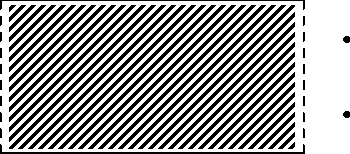
\includegraphics[height=1.8cm]{images/figuresasy-1}
      \caption{$A$}
    \end{subfigure}%
    \qquad
    \begin{subfigure}[b]{0.3\textwidth}
      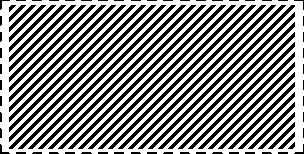
\includegraphics[height=1.8cm]{images/figuresasy-2}
      \caption{int($A$) --- l'intérieur de $A$}
    \end{subfigure}%
    \qquad
    \begin{subfigure}[b]{0.3\textwidth}
      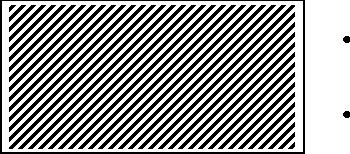
\includegraphics[height=1.8cm]{images/figuresasy-3}
      \caption{$\bar{A}$ --- la fermeture de $A$}
    \end{subfigure}

    \begin{subfigure}[b]{0.3\textwidth}
      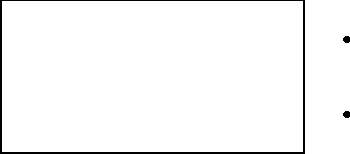
\includegraphics[height=1.8cm]{images/figuresasy-4}
      \caption{fr($A$) --- la frontière de $A$}
    \end{subfigure}%
    \qquad
    \begin{subfigure}[b]{0.3\textwidth}
      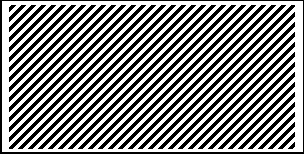
\includegraphics[height=1.8cm]{images/figuresasy-5}
      \caption{Les points limites ou d'accumulation de $A$}
    \end{subfigure}%
    \qquad
    \begin{subfigure}[b]{0.3\textwidth}
      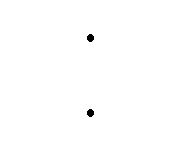
\includegraphics[height=1.8cm]{images/figuresasy-6}
      \caption{Les points isolés de $A$}
    \end{subfigure}
    \caption{Les divers ensembles}
    \label{fig:ensembles}
\end{figure}


\subsection{Ensembles ouverts, bornés et complémentaires}

\begin{mydef}
    $A$ est un ensemble \textbf{borné} 
    s'il existe une boule ouverte qui contient $A$;
    sinon, l'ensemble $A$ est dit \textbf{non-borné}.
\end{mydef}

\begin{mydef}
    Un ensemble est \textbf{ouvert} si et seulement si
    \[ A = \newint A \]
    Un ensemble est \textbf{fermé} si et seulement si
    \[ A = \bar{A} \]
\end{mydef}

\begin{myrem}
    L'ensemble vide $\emptyset$ et l'espace complet $\Rn$ 
    sont à la fois ouverts et fermés.
\end{myrem}

\begin{myprop}\InsertTheoremBreak
    \begin{itemize}
        \item La fermeture d'un ensemble est 
            le plus petit ensemble fermé contenant cet ensemble,
        \item L'intérieur d'un ensemble est 
            le plus grand ensemble ouvert contenu dans cet ensemble.
    \end{itemize}
\end{myprop}

\begin{mydef}
    Le complémentaire d'un ensemble $A \subseteq \Rn$ est 
    l'ensemble des points n'appartenant pas à $A$,
    c'est-à-dire $\Rn \setminus A$.
\end{mydef}

\begin{mytheo}
    Le complémentaire d'un ensemble ouvert est toujours un ensemble fermé;
    celui d'un ensemble fermé est toujours ouvert.
\end{mytheo}

\subsection{Limites}

Dans cette partie, on considère $f : A \subseteq \R^n \to \R$ 

\begin{mydef}[Limite d'une fonction à plusieurs variables]
    On peut définir la limite de $f$ en tout point de la \emph{fermeture} de 
    son domaine (éventuellement hors de $A$).
    Si $a$ est un point isolé de $A$, alors
    \[ \lim_{x \to a} f(x) = f(a) \]
    Si $a$ est un point limite de $A$, alors
    \[ \lim_{x \to a} f(x) = L \]
    si et seulement si $\forall \epsilon >0, \exists \delta > 0$ 
    tel que $x \in A$ et
    \[ 0 < \norm{x - a} < \delta \Rightarrow \abs{f(x) - L} < \epsilon \]
    Si la fonction est vectorielle et que $a$ est un point limite de $A$, alors
    \[ \lim_{x \to a} f(x) = L \]
    si et seulement si $\forall \epsilon >0, \exists \delta > 0$ tel que $x \in A$ et
    \[ 0 < \norm{x - a} < \delta \Rightarrow \norm{f(x) - L} < \epsilon \]
    (comme on dit $0 < \norm{x - a}$, la valeur de $f(a)$, si elle existe, 
    n'influe en rien la limite).

    Si on écrit $f$ sous la forme $f = (f_1 , \dots , f_n)$ où chaque $f_i$ est
    une fonction scalaire, alors la limite de $f$ existe si et seulement si la 
    limite de chaque $f_i$ existe
    \[ \lim_{x \to a} f(x) = \left( \lim_{x \to a} f_1(x), 
    \lim_{x \to a} f_2(x), \dots , \lim_{x \to a} f_n(x) \right)^T \]
\end{mydef}

\begin{myprop}[Condition nécessaire et suffisante à l'existence d'une limite]
    Soient $a \in \bar{A}$ et $B = B(a; r)$ une boule ouverte centrée en $a$.
    Soit $f_B$ une restriction de la fonction $f$ à $B$.
    \( \lim_{x \to a}f(x) \)
    existe si et seulement si
    \( \lim_{x \to a}f_B(x) \)
    existe et si elles existent elles sont égales.
\end{myprop}

\begin{myprop}[Condition nécessaire mais \textbf{pas} suffisante à l'existence 
    d'une limite]
    \label{prop:path}
    Soient $B$ un sous-ensemble de $A$ et $a \in \bar{B}$.
    Soit $f_B$ une restriction de la fonction $f$ à $B$.
    Si
    \( \lim_{x \to a}f(x) \)
    existe, alors
    \( \lim_{x \to a}f_B(x) \)
    existe et elles sont égales.
    \subparagraph{Remarques}
    \begin{itemize}
        \item On fait souvent ces restrictions le long de chemins: des 
            (demi-)droites passant par $a$ ou d'autres courbes;
        \item certaines fonctions n'ont pas de limite en un point alors que 
            toutes les restrictions à des droites passant par
            ce point admettent une même limite;
        \item si $\lim_{x \to a}f_B(x)$ n'existe pas, alors 
            $\lim_{x \to a} f(x)$ n'existe pas non plus.
        \item si $\lim_{x \to a}f_{B_1}(x)$ et $\lim_{x \to a}f_{B_2}(x)$ 
            existent et sont différentes, alors $\lim_{x \to a} f(x)$ n'existe 
            pas.  Avant de se lancer dans le calcul d'une limite, il est 
            intéressant de vérifier son existence. Pour ce faire, on peut la 
            calculer le long de chemins génériques comme $y = mx + p$ et 
            $y = mx^2$, si la limite dépend de $m$, alors elle est différente 
            pour chaque chemin et donc n'existe pas. Si elle ne dépend pas de 
            $m$, alors on peut \emph{supposer} qu'elle existe et se lancer dans 
            son calcul.
    \end{itemize}
\end{myprop}

\begin{myprop}[Recollement (condition nécessaire et suffisante)]
    \label{prop:rec}
    Soit $A = A_1 \cup A_2$ ; soient $f_1$, $f_2$ les restrictions respectives 
    de $f$ à $A_1$ et $A_2$. Si $a \in \bar{A_1}$ et $a \in \bar{A_2}$, alors
    \[ \lim_{x \to a}f(x) = L \Leftrightarrow \left\{
    \begin{array}{l}
        \lim_{x \to a} f_1(x) = L \\
        \lim_{x \to a}f_2(x) = L
    \end{array} \right. \]
\end{myprop}

\begin{myrem}
    La différence entre la Propriété~\ref{prop:path} et la 
    Propriété~\ref{prop:rec} c'est que si vous coupez le domaine $A$ en un 
    nombre \emph{fini} de restrictions dont l'union redonne $A$,
    alors vous avez la condition suffisante, sinon, vous ne l'avez pas.
\end{myrem}

\begin{myform}[Combinaisons algébriques]
    Les quatre opérations classiques ($+$, $-$, $\times$, $\div$) sont 
    possibles, mais \textbf{pas} la composition de limites.
\end{myform}

\begin{myprop}[Positivité] \InsertTheoremBreak
    \begin{itemize}
        \item $f(x) \geq 0 \Rightarrow \lim_{x \to a} f(x) \geq 0$ ;
        \item $f(x) > 0 \Rightarrow \lim_{x \to a} f(x) \geq 0$ ;
        \item $f(x) \leq g(x) \Rightarrow 
            \lim_{x \to a} f(x) \leq \lim_{x \to a} g(x)$.
    \end{itemize}
    Fonctionne aussi dans un voisinage de $a$.
\end{myprop}

\begin{myprop}[Étau (condition suffisante)]
    Si $g \leq f \leq h$ et que $\lim_{x \to a} g(x) = \lim_{x \to a} h(x) = L$
    alors \[ \lim_{x \to a} f(x) = L. \]
    Fonctionne aussi dans un voisinage de $a$.
\end{myprop}

\begin{myform}[Applications de l'étau]\InsertTheoremBreak
    \begin{itemize}
        \item Si $f \rightarrow 0$, alors $|f| \rightarrow 0$ ;
        \item si $f \to 0$, et que $g$ est bornée, 
            alors $\lim_{x \to a} (g \cdot f) = 0$.
    \end{itemize}
\end{myform}

\begin{myrem}[Limites et coordonnées polaires]
    Il est parfois utile de passer par les coordonnées polaires pour calculer une limite. Il suffit
    alors de poser $x = \rho \cos \theta$ et $y = \rho \sin \theta$. Dans la plupart des cas, on
    utilisera les coordonnées polaires lorsque l'expression $x^2 + y^2$ apparaît. En effet, en
    utilisant les coordonnées polaires, l'expression devient simplement $\rho^2$.
    Attention cependant, effectuer un tel changement de variables revient à faire une composition.
    Il faut donc changer les points où on évalue la limite. Par exemple : la limite pour
    $(x, y) \rightarrow (0, 0)$ de $f(x, y)$ devient la limite pour $\rho \rightarrow 0$ et $\theta$
    variable de $f(\rho \cos \theta, \rho \sin \theta)$.
\end{myrem}

\begin{mydef}[Continuité]
    Une fonction $f : A \subseteq \R^n \rightarrow \R^m$ est continue en $a \in A$ si et seulement si
    \[ \lim_{x \rightarrow a}f(x) = f(a) \]
\end{mydef}

\begin{myprop}\InsertTheoremBreak
    \begin{itemize}
        \item Si $f$ et $g$ sont continues en $a$, alors
            $f \pm g$ et $f \cdot g$ sont continues en $a$.
            Si $g(a) \neq 0$, alors $\frac{f}{g}$ est continue en $a$ ;
        \item si $f$ est continue en $a$ et $g$ en $f(a)$,
            $g \circ f$ est continue en $a$ ;
        \item une fonction vectorielle est continue si et seulement si chaque composante est continue.
    \end{itemize}
\end{myprop}

\begin{myrem}
    Une fonction est toujours continue en un point isolé de $A$.
\end{myrem}

\begin{myrem}
    Les quatres opérations classiques \emph{ainsi que la composition} préservent la continuité.
\end{myrem}


%%%%%%%%%%%%%%%%%%%%%%%%%%%%%%%%%%%%%%%%%%%%%%%%%%%%%%%%%%%%%%%%%%%%%%%%%%%%%%%%%%%%%%%
%%%%%%%%%%%%%%%%%%%%%%%%%%%%%%%%%%%%%%%%%%%%%%%%%%%%%%%%%%%%%%%%%%%%%%%%%%%%%%%%%%%%%%


\section{Dérivées directionnelles et partielles}

\begin{mydef}
    Une \textbf{direction} de $\Rn$ est un vecteur $d \in \Rn$ tel que 
    $\norm{d} = 1$.
\end{mydef}

\begin{mydef}[Dérivée directionnelle] Soient $f : A \subseteq \R^n \to \R^m$, $a$ un point intérieur de $A$, $d \in \R^n$ une direction. La dérivée directionnelle de $f$ en $a$ dans la direction $d$ est notée $D_df(a)$ et vaut, si elle existe, la limite suivante
    \[ D_df(a) = \lim_{t \to 0} \frac{f(a+td) - f(a)}{t} \]
    Graphiquement, il s'agit de la pente de la tangente au point $a$ de la coupe verticale du graphe
    par la droite $a+td$.
\end{mydef}

\begin{myform}[Approximation linéaire dans une direction]
    \[ f(a+td) \approx f(a) + t D_df(a) \]
\end{myform}

\begin{myform}
    \begin{eqnarray*}
        D_d(g+h)(a) &=& D_dg(a) + D_d h(a)\\
        D_d(gh)(a) &=& D_dg(a)h(a) + g(a)D_dh(a)\\
        D_d(g\circ h)(a) &=& g'(h(a))D_dh(a)\\
        D_df(a) &=& (D_df_1(a), D_df_2(a), \dots, D_df_m(a))^T
    \end{eqnarray*}
\end{myform}

\begin{mydef}[Dérivée partielle]
    C'est la dérivée directionnelle le long d'un axe.
    Soit une fonction $f : A\subseteq \R^n \to \R^m$ et $a$ un point intérieur de $A$. La dérivée partielle de $f$ par rapport à une de ses variables $x_i$ est la dérivée directionnelle de $f$ au point $a$ dans la direction
    \[ e^{(i)} = (\underbrace{0; \dots; 0}_{i-1\text{ fois }0}; 1; 0; \dots; 0)^T \]
    et se note
    \[ \frac{\pa f}{\pa x_i}(a) \eqdef D_{e^{(i)}} f(a) = \lim_{t \to 0} \frac{f(a+te^{(i)})
    - f(a)}{t}\]
\end{mydef}

\begin{myrem}[Continuité et dérivées directionnelles]
    L'existence de toutes les dérivées directionnelles 
    (et donc \textit{a fortiori} partielles) en un point n'implique pas la continuité.
\end{myrem}

\begin{myform}[Calcul des dérivées partielles] Pour calculer les dérivées partielles de $f$ selon une de ses variables $x_i$, on fixe toutes les autres variables et on calcule la dérivée partielle comme la dérivée d'une fonction à une seule variable ($x_i$).
\end{myform}

\begin{mydef}[Dérivées partielles d'ordre supérieur]
    L'existence des $i$\ieme{} dérivées partielles définit une fonction
    \[ \frac{\pa^i f}{\pa x^i} : \newint A \subseteq \R^n \to \R : x \to \frac{\pa^i f}{\pa x^i}(x) \]
\end{mydef}

%%%%%%%%%%%%%%%%%%%%%%%%%%%%%%%%%%%%%%%%%%%%%%%%%%%%%%%%%%%%%%%%%%%%%%%%%%%%%%%%%%%%%%%
%%%%%%%%%%%%%%%%%%%%%%%%%%%%%%%%%%%%%%%%%%%%%%%%%%%%%%%%%%%%%%%%%%%%%%%%%%%%%%%%%%%%%%

\section{Différentielle}

\subsection{Définitions}

\begin{mydef}[Différentielle]
    Soit une fonction $f : A \subseteq \R^n \to \R^m$, $a \in \R^n$ un point intérieur de $A$ et $h = (\dif x_1, \dots, \dif x_n)$ un vecteur de $\R^n$. La fonction $f$ est différentiable en $a$ si et seulement si il existe une application linéaire $L : \R^n \to \R^m$ telle que
    \[ \lim_{h \to 0} \frac{f(a+h) - f(a) - L(h)}{\norm{h}} = 0 \]
    Si cette application linéaire $L$ existe, alors on l'appelle différentielle de $f$ en $a$ et elle se note
    \[ L = \dif f_a \]
\end{mydef}

\begin{myprop}[Approximation locale linéaire]
    Soit $f : A \subseteq \R^n \to \R^m$ et $a$ un point intérieur à $A$. $f$ est différentiable si et seulement si il existe une application linéaire $L : \R^n \to \R^m$ et une fonction $r : \R^n \to \R^m$ telles que
    \[ f(a+h) = f(a) + L(h) + \norm{h} r(h) \]
    et
    \[ \lim_{h \to 0}r(h) = 0 \]
\end{myprop}

\begin{myprop}[Continuité]
    La différentiabilité garantit la continuité\footnote{Cela se prouve assez facilement
    en utilisant la définition de la continuité et la propriété ``Approximation locale linéaire''.}.
\end{myprop}

\begin{myform}[Lien avec les dérivées partielles] On a les formules
    \[ \dif f_a : (\dif x_1 , \dots , \dif x_n) \to \sum_{i=1}^n \frac{\pa f}{\pa x_i}(a) \dif x_i \]
    \[ \frac{\pa f}{\pa x_i}(a) = \dif f_a(e^{(i)}) \]
\end{myform}

\begin{myform}
    Si $f$ est \textbf{différentiable} au point $a$, on a
    \[ D_df(a) = \dif f_a(d) \]
    Si $f$ n'est \textbf{pas différentiable} au point $a$, on n'a \textbf{pas} spécialement
    \[ D_df(a) = \sum_{i = 1}^n \frac{\partial f}{\partial x_i}(a)d_i \]
    Si vous utilisez cette formule, il ne faut pas oublier de mentionner le fait que $f$ est différentiable au point $a$
    et de le montrer si ce n'est pas déjà fait.
\end{myform}

\begin{myprop}[Condition suffisante pour la différentiabilité] Soient une fonction $f : A \subseteq \R^n \to \R^m$ et $a$ un point intérieur à $A$. $f$ est différentiable si
    \begin{itemize}
        \item toutes les dérivées partielles de $f$ \emph{existent} en $a$ ;
        \item toutes les dérivées partielles \emph{sauf au plus une} sont continues dans un voisinage de $a$ (dans \emph{une} boule ouverte centrée en $a$).
    \end{itemize}
\end{myprop}

\subsection{Procédure de calcul de la différentielle}
\begin{enumerate}
    \item Calculer toutes les dérivées partielles de $f$ au point $a$ (règle usuelle ou définition);
        si l'une d'entre elles n'existe pas, $f$ n'est pas différentiable au point $a$
    \item Écrire une expression candidate pour la différentielle
        \[ \dif f_a(\dif x_1, \dif x_2, \dots, \dif x_n) = \sum_{i = 1}^n \frac{\partial f}{\partial x_i}(a) \dif x_i \]
    \item Vérifier que cette expression est correcte
        \begin{enumerate}
            \item Soit en prouvant séparément que la fonction est différentiable en $a$
                \begin{itemize}
                    \item[$\bullet$] en montrant la continuité des dérivées partielles dans un voisinage de $a$;
                    \item[$\bullet$] ou en combinant des fonctions connues différentiables pour obtenir $f$.
                \end{itemize}
                \begin{itemize}
                    \item Si c'est possible, l'expression candidate est bien la différentielle;
                    \item mais si ce n'est pas possible, on ne peut rien en conclure.
                \end{itemize}
            \item Soit en remplaçant $L(h)$ par l'expression candidate dans la définition
                \begin{itemize}
                    \item Si définition vérifiée, l'expression candidate est bien la différentielle;
                    \item Si définition pas vérifiée (limite différente de 0 ou inexistante),
                        on est bien sûr que $f$ n'est pas différentiable au point $a$.
                \end{itemize}
        \end{enumerate}
\end{enumerate}

\subsection{Formules de calcul}

\begin{myprop}
    Les opérations usuelles (somme, produit, composition, etc.) préservent la différentiabilité
    (à l'intérieur du domaine pertinent).

    Ceci permet de prouver la différentiabilité de la plupart des fonctions classiques,
    à l'exception des points délicats
    (dénominateur nul, fonctions définies à l'aide de cas par morceaux),
    à l'aide de combinaisons de fonctions simples dont la différentiabilité est prouvée:
    \begin{enumerate}
        \item les fonctions linéaires et affines
        \item les fonctions dérivables à une variable
    \end{enumerate}
\end{myprop}

\noindent
\begin{tabularx}{1.0\textwidth}{|S X|S X|}
    \hline
    Fonction & Différentielle (au point $a$, évaluée en $h$)\\
    \hline\hline
    $ \displaystyle M \cdot x \;\text{avec}\; M \in \R^{m \times n} $ & $\displaystyle M \cdot h $\\
    \hline
    $ \displaystyle M \cdot x + p $ & $\displaystyle  M \cdot h $ \\
    \hline
    $ \lambda \cdot f(x) \;\text{avec}\; \lambda \in \R $ & $\displaystyle \lambda \cdot \dif f_a (h) $ \\
    \hline
    $ \displaystyle M \cdot f(x) \;\text{avec}\; M \in \R^{p \times m}$ & $\displaystyle M \cdot \dif f_a (h)$ \\
    \hline
    $ \displaystyle f(x) + g(x) $ & $ \displaystyle \dif f_a (h) + \dif g_a (h) $ \\
    \hline
    $ \displaystyle f(x)\cdot g(x) $ & $\displaystyle  g(a) \cdot \dif f_a(h) + f(a) \cdot \dif g_a(h) $ \\
    \hline
    $ \displaystyle \frac{f(x)}{g(x)} $ & $\displaystyle  \frac{g(a) \cdot \dif f_a(h) - f(a) \cdot \dif g_a(h) }{g(a)^2} $ \\
    \hline
    $ \displaystyle (f(x)|g(x)) $ & $\displaystyle  (\dif f_a(h) | g(a) ) + (f(a)|\dif g_a(h)) $ \\
    \hline
    $ \displaystyle (f \circ g)(x) $ & $\displaystyle  \dif f_{g(a)} \circ \dif g_a(h) $ \\
    \hline
\end{tabularx}

%%%%%%%%%%%%%%%%%%%%%%%%%%%%%%%%%%%%%%%%%%%%%%%%%%%%%%%%%%%%%%%%%%%%%%%%%%%%%%%%%%%%%%%
%%%%%%%%%%%%%%%%%%%%%%%%%%%%%%%%%%%%%%%%%%%%%%%%%%%%%%%%%%%%%%%%%%%%%%%%%%%%%%%%%%%%%%

\section{Plans et vecteurs tangents, gradient}

\subsection{Courbes et surfaces paramétrées}

\begin{mydef}[Courbe paramétrée]
    Soit une courbe paramétrée dans $\R^m$ décrite par $f : A \subseteq \R \to \R^m$
    \[ \mathcal{C} = \{ f(t) \suchthat t \in A \subseteq \R \} \subseteq \R^m \]
\end{mydef}

\begin{myform}[Droite tangente]
    Si $f$ est différentiable, alors la droite tangente à la courbe $\mathcal{C}$ en $f(a)$ a pour équation paramétrique
    \[ t \to f(a) + t f'(a) \]
    Où $f'(a)$ est le vecteur tangent à $\mathcal{C}$ en $a$
    Dans ce cas,
    \[ f(a + t) \approx f(a) + \dif f_a(t) = f(a) + t f'(a) \]
\end{myform}

\begin{mydef}[Surface paramétrée]
    Une surface paramétrée de $\R^m$ décrite par $f : A \subseteq \R^2 \to \R^m$ est
    \[ \mathcal{S} = \{ f(u,v) \suchthat (u,v) \in A \subseteq \R^2 \} \subseteq \R^m \]
\end{mydef}

\begin{myform}[Plan tangent]
    Si $f$ est différentiable en $(a,b)$, le plan tangent à $f$ au point $(a,b)$ est paramétré par
    \[ (u,v) \to f(a,b) + (u-a) \frac{\pa f}{\pa x_1} (a,b) + (v-b) \frac{\pa f}{\pa x_2}(a,b) \]
\end{myform}

\subsection{Gradient}

\begin{mydef}[Gradient] Soit $f : A \subseteq \R^n \to \R$ une fonction scalaire différentiable en $a$, le gradient est un vecteur ligne à $n$ composantes
    \[ (\newgrad f)(a) = \nabla f(a) = \left( \frac{\pa f}{\pa x_1}(a) , \dots, \frac{\pa f}{\pa x_n}(a) \right) \]
\end{mydef}

\begin{myform} On a que
    \[ D_df(a) = \dif f_a(d) = \nabla f(a) d \]
\end{myform}

\begin{myprop} Le gradient est parallèle à la direction de plus forte pente,
    celle où $D_df(a)$ est maximal
    \footnote{\c{C}a peut se prouver aisément en majorant $D_df(a)$ par l'inégalité de Cauchy et en remarquant qu'on doit être dans le cas d'égalité pour être maximum.}.
    Il est aussi orthogonal à tout vecteur tangent à la courbe de niveau de $f$ passant par le point $a$.
\end{myprop}

\subsection{Courbes et surfaces définies par un graphe}

\begin{myform}[Plan tangent à un graphe]
    Soit une fonction scalaire $f : A \subseteq \R^n \to \R$ différentiable en $a$, un point intérieur de $A$. Le plan tangent $z$ au point $(a,f(a))$ est
    \begin{align*}
        z & = f(a) + \frac{\pa f}{\pa x_1}(a)(x_1 - a_1) + \cdots + \frac{\pa f}{\pa x_n}(a) (x_n - a_n) \\
        & = f(a) + \dif f_a(x-a) \\
        & = f(a) + \nabla f(a)(x-a)
    \end{align*}
    La normale de ce plan tangent est
    \[
    \begin{pmatrix}
        \nabla f(a) & -1
    \end{pmatrix}
    \]
\end{myform}

%%%%%%%%%%%%%%%%%%%%%%%%%%%%%%%%%%%%%%%%%%%%%%%%%%%%%%%%%%%%%%%%%%%%%%%%%%%%%%%%%%%%%%%
%%%%%%%%%%%%%%%%%%%%%%%%%%%%%%%%%%%%%%%%%%%%%%%%%%%%%%%%%%%%%%%%%%%%%%%%%%%%%%%%%%%%%%

\section{Théorème des accroissement finis}

\begin{mytheo}[Théorème des accroissements finis] 
    Soit une fonction scalaire $f : A \subseteq \R^n \to \R$ continue 
    sur l'intervalle fermé $\closedItv{a}{b}$ 
    et différentiable sur l'intervalle $\openItv{a}{b}$
    \footnote{La notion d'intervalle peut être généralisée à $\Rn$ : 
        l'intervalle ouvert (fermé) $\openItv{a}{b}$ est le segment ouvert (fermé) 
    entre $a$ et $b$.}
    , $\exists c \in \openItv{a}{b}$ tel que
    \[ f(b) - f(a) = \dif f_c(b-a) \]
\end{mytheo}

\begin{mytheo}[Théorème des accroissements finis (formulation équivalente
        \footnote{Elle s'obtient de la formulation précédente en posant 
        $b = a+h$ et en repèrant la position de $c$ dans 
        $\openItv{a}{b}$ par $c = a +\theta h$.})]
Soit $f$ une fonction scalaire. $\exists 0 < \theta < 1$ tel que
    \[ f(a+h) = f(a) + \dif f_{a + \theta h}(h) = f(a) + \nabla f(a + \theta h)h \]
\end{mytheo}

\begin{myprop}[Pour les fonctions vectorielles]
    On n'a pas le théorème des accroissements finis, mais on a que
    $\exists c \in \openItv{a}{b}$ tel que
    \[ \norm{f(b) - f(a)} \leq \norm{\dif f_c(b-a)} \]
\end{myprop}

%%%%%%%%%%%%%%%%%%%%%%%%%%%%%%%%%%%%%%%%%%%%%%%%%%%%%%%%%%%%%%%%%%%%%%%%%%%%%%%%%%%%%%%
%%%%%%%%%%%%%%%%%%%%%%%%%%%%%%%%%%%%%%%%%%%%%%%%%%%%%%%%%%%%%%%%%%%%%%%%%%%%%%%%%%%%%%

\section{Classes de fonctions}

\begin{mydef}[Classe de fonctions $\mathcal{C}^k$]
    Une fonction $f$ est dite de classe $\mathcal{C}^k$ sur un ensemble ouvert 
    $A$ si et seulement si toutes ses dérivées partielles $k$\ieme{} existent 
    \emph{et sont continues} sur $A$. On écrit alors
    \[ f \in \mathcal{C}^k(A) \]
\end{mydef}

\begin{myprop}[Classe de fonction] On a les inclusions suivantes
    \[ \mathcal{C}^{\infty}(A) \subset \dots \subset \mathcal{C}^3(A) \subset \mathcal{C}^2(A) \subset \mathcal{C}^1(A) \subset \mathcal{C}^0(A) \]
\end{myprop}

%%%%%%%%%%%%%%%%%%%%%%%%%%%%%%%%%%%%%%%%%%%%%%%%%%%%%%%%%%%%%%%%%%%%%%%%%%%%%%%%%%%%%%%
%%%%%%%%%%%%%%%%%%%%%%%%%%%%%%%%%%%%%%%%%%%%%%%%%%%%%%%%%%%%%%%%%%%%%%%%%%%%%%%%%%%%%%

\section{Matrices hessiennes et jacobiennes}

\begin{mydef}[Matrice hessienne]
    Soit $f : A \subseteq \R^n \to \R$ et $a$ un point intérieur de $A$. Si toutes les dérivées partielles secondes existent en $a$, la matrice hessienne est la matrice carrée de dimension $n$ suivante
    \[ Hf(a) = \begin{pmatrix}
        \frac{\pa^2 f}{\pa x_1^2}(a) & \frac{\pa^2 f}{\pa x_2 x_1}(a) & \cdots & \frac{\pa^2 f}{\pa x_n \pa x_1}(a) \\
        \frac{\pa^2 f}{\pa x_1 \pa x_2}(a) & \frac{\pa^2 f}{\pa x_2^2}(a) & \cdots & \frac{\pa^2 f}{\pa x_n \pa x_2}(a) \\
        \vdots & \vdots & \ddots & \vdots \\
        \frac{\pa^2 f}{\pa x_1 \pa x_n}(a) & \frac{\pa^2 f}{\pa x_2 \pa x_n}(a) & \cdots & \frac{\pa^2 f}{\pa x_n^2}(a) \\
    \end{pmatrix} \]
\end{mydef}

\begin{myprop}[Matrice symétrique]
    Soit $f : A \subseteq \R^n \to \R$.
    Si $f \in \mathcal{C}^2(A)$, alors
    \[ \frac{\pa^2 f}{\pa x_j \pa x_i}(a) = \frac{\pa^2 f}{\pa x_i \pa x_j}(a) \]
    pour tout $a \in A$ et pour tous $1 \leq i,j \leq n$. 
    Dans ce cas, la matrice hessienne est symétrique.
    Autrement dit, la hessienne est symétrique si ses fonctions sont continues.
\end{myprop}

\begin{myprop}[Ordres supérieurs]
    Si une fonction est de classe $\mathcal{C}^k$ alors on peut permuter l'ordre de dérivation des variables pour les dérivées partielles d'ordre $k$.
\end{myprop}

\begin{mydef}[Matrice jacobienne]
    Soit une fonction $f : A \subseteq \R^n \to \R^m$ différentiable en un point $a$ intérieur à $A$. La matrice jacobienne est une matrice $m \times n$ :
    \[ Jf(a) =
    \begin{pmatrix}
        \frac{\pa f_1}{\pa x_1}(a) & \frac{\pa f_1}{\pa x_2}(a) & \cdots & \frac{\pa f_1}{\pa x_n}(a) \\
        \frac{\pa f_2}{\pa x_1}(a) & \frac{\pa f_2}{\pa x_2}(a) & \cdots & \frac{\pa f_2}{\pa x_n}(a) \\
        \vdots & \vdots & \ddots & \vdots \\
        \frac{\pa f_m}{\pa x_1}(a) & \frac{\pa f_m}{\pa x_2}(a) & \cdots & \frac{\pa f_m}{\pa x_n}(a) \\
    \end{pmatrix} \text{avec } f =
    \begin{pmatrix}
        f_1 \\ f_2 \\ \vdots \\ f_m
    \end{pmatrix} \]
\end{mydef}

\begin{myform}[Lien avec gradient, dérivées partielles, ...]
    On a les formules suivantes :
    \[ Jf(a) =
    \begin{pmatrix} \nabla f_1(a) \\ \nabla f_2(a) \\ \vdots \\ \nabla f_m(a)
    \end{pmatrix} \]
    \[ Jf(a) =
    \begin{pmatrix} \frac{\pa f}{\pa x_1}(a) & \frac{\pa f}{\pa x_2}(a) & \cdots & \frac{\pa f}{\pa x_n}(a)
    \end{pmatrix} \]
    Pour chaque composante scalaire d'une fonction vectorielle
    \[ \dif f_a(h) = Jf(a) h \]
    La matrice jacobienne est donc la matrice associée à l'application linéaire $\dif f_a$.
    Pour une fonction à une seule variable représentant une courbe paramétrée de $\R^n$ :
    \[ Jf(a) = f'(a) \]
\end{myform}

%%%%%%%%%%%%%%%%%%%%%%%%%%%%%%%%%%%%%%%%%%%%%%%%%%%%%%%%%%%%%%%%%%%%%%%%%%%%%%%%%%%%%%%
%%%%%%%%%%%%%%%%%%%%%%%%%%%%%%%%%%%%%%%%%%%%%%%%%%%%%%%%%%%%%%%%%%%%%%%%%%%%%%%%%%%%%%

\section{Développements de Taylor}

\begin{myform}[Développement avec reste d'ordre 1]
    Soit $A \subseteq \R^n$ un ensemble ouvert, $f : A \subseteq \R^n \to \R$ une fonction scalaire de classe $\mathcal{C}^1$, $a \in \R^n$ un point de $A$ et $h$ un vecteur de $\R^n$ tel que $[a, a+h] \subseteq A$. $\exists 0 < \theta < 1$ tel que
    \begin{align*}
        f(a+h) & = f(a) + \nabla f(a+\theta h)h \\
        & = f(a) + \sum_{i =1}^n \frac{\pa f}{\pa x_i} (a+\theta h)h_i
    \end{align*}
    C'est le théorème des accroissement finis.
\end{myform}

\begin{myform}[Développement avec reste d'ordre 2]
    Soit $f$ une fonction de classe $\mathcal{C}^2$.
    $\exists 0 < \theta < 1$ tel que
    \begin{align*} f(a+h) & = f(a) + \nabla f(a) h + \frac12 h^T Hf(a+\theta h) h \\
        & = f(a) + \sum_{i=1}^n \frac{\pa f}{\pa x_i}(a)h_i + \frac12 \sum_{i=1}^n \sum_{j=1}^n \frac{\pa^2 f}{\pa x_i \pa x_j} (a+ \theta h) h_i h_j
    \end{align*}
\end{myform}

\begin{myform}[Développement avec reste d'ordre 3]
    Soit $f$ une fonction de classe $\mathcal{C}^3$.
    $\exists 0 < \theta < 1$ tel que
    \begin{eqnarray*}
        f(a+h) &=& f(a) + \sum_{i=1}^n \frac{\pa f}{\pa x_i}(a)h_i
        + \frac 12 \sum_{i=1}^n \sum_{j=1}^n \frac{\pa^2 f}{\pa x_i \pa x_j} (a) h_i h_j \\
        && + \frac{1}{3!} \sum_{i=1}^n \sum_{j=1}^n \sum_{k=1}^n \frac{\pa^3 f}{\pa x_i \pa x_j \pa x_k}(a+\theta h)h_i h_j h_k
    \end{eqnarray*}
    Dans le cas d'une fonction $f$ à 2 variables $x, y$, le reste du développement de Taylor s'écrit
    \[
    \frac{1}{6}
    \left(
    \frac{\pa^3 f}{\pa x^3}(c)h_1^3
    + 3\frac{\pa^3 f}{\pa x^2\pa y}(c)h_1^2h_2\\
    + 3\frac{\pa^3 f}{\pa x\pa y^2}(c)h_1h_2^2
    + \frac{\pa^3 f}{\pa y^3}(c)h_2^3
    \right)
    \]
    où $a + \theta h$ a été remplacé par $c$ pour plus de concision.
\end{myform}

\begin{myform}[Développement de Taylor \emph{limité} à l'ordre 1]
    Soit $f$ une fonction de classe $\mathcal{C}^1$. L'approximation d'ordre 1 de la fonction $f$ au point $a$
    \[
    f(a+h) \approx f(a) + \sum_{i =1}^n \frac{\pa f}{\pa x_i} (a)h_i
    \]
\end{myform}

%%%%%%%%%%%%%%%%%%%%%%%%%%%%%%%%%%%%%%%%%%%%%%%%%%%%%%%%%%%%%%%%%%%%%%%%%%%%%%%%%%%%%%%
%%%%%%%%%%%%%%%%%%%%%%%%%%%%%%%%%%%%%%%%%%%%%%%%%%%%%%%%%%%%%%%%%%%%%%%%%%%%%%%%%%%%%%

\section{Composition (\emph{chain rule})}

\begin{myform}[\emph{Chain rule}]
    On peut écrire la matrice jacobienne d'une composée comme un produit matriciel:
    \[ J(g \circ f)(a) = Jg(f(a)) \cdot Jf(a) \]
    Si on explicite les composantes $f_1, f_2, \dots , f_m$ de $f$ avec
    \[ g(f(x)) = g( f_1(x_1, \dots, x_n), f_2(x_1, \dots, x_n), \dots, f_m(x_1, \dots, x_n)) \]
    et $g$ définie de sorte qu'on ait $g : (y_1, y_2, \dots , y_m) \rightarrow g(y_1, y_2, \dots, y_m)$. Donc $x$ sont les variables naturelles de $f$ et $y$ celles de $g$.
    Alors on a la formule\footnote{Notez la différence par rapport aux slides du cours, où les $y_1, y_2, \dots, y_n$ remplacent les $x_1, x_2, \dots, x_n$ pour ne pas les confondre avec les variables de $f$}
    \[ \frac{\pa (g \circ f)}{\pa x_i}(a) = \frac{ \pa g}{\pa y_1}(f(a)) \frac{\pa f_1}{\pa x_i}(a) + \frac{ \pa g}{\pa y_2}(f(a)) \frac{\pa f_2}{\pa x_i}(a) + \cdots + \frac{ \pa g}{\pa y_m}(f(a)) \frac{\pa f_m}{\pa x_i}(a) \]
\end{myform}

%%%%%%%%%%%%%%%%%%%%%%%%%%%%%%%%%%%%%%%%%%%%%%%%%%%%%%%%%%%%%%%%%%%%%%%%%%%%%%%%%%%%%%%
%%%%%%%%%%%%%%%%%%%%%%%%%%%%%%%%%%%%%%%%%%%%%%%%%%%%%%%%%%%%%%%%%%%%%%%%%%%%%%%%%%%%%%

\section{Optimisation}

On ne parlera ici que de fonction scalaire car il n'y a pas d'ordre dans $\Rn$ avec $n > 1$.
On ne peut pas dire $a < b$ si $a, b \in \Rn$, ce n'est pas défini.

\subsection{Définitions}

\begin{mydef}[Extremum global] Un extremum global est un point où $f$ prend une valeur extrême ; c'est à dire un point $a$ tel que
    \[ f(a) \begin{array}{l} \geq \\ \leq \end{array} f(x) \; \forall x \in A \begin{array}{l} \text{(maximum)} \\ \text{(minimum)}
    \end{array} \]
\end{mydef}

\begin{mydef}[Extremum local] Un extremum local est un point où $f$ prend une valeur extrême sur un voisinage; c'est à dire un point $a$ tel que
    \[ \exists r >0 \; \text{tel que} \; f(a) \begin{array}{l} \geq \\ \leq \end{array} f(x) \; \forall x \in B(a;r) \cap A \begin{array}{l} \text{(maximum)} \\ \text{(minimum)}
    \end{array} \]
\end{mydef}

\begin{mydef}[Extremum local libre]
    Un extremum local libre de $f$ est un extremum local $a \in \newint A$.
\end{mydef}

\begin{mydef}[Extremum local lié]
    Un extremum local lié de $f$ est un extremum local 
    $a \in \newfr A \cap A = A \setminus \newint A$.
\end{mydef}

\begin{mydef}[Point-selle]
    Un point-selle (parfois aussi appelé un ``col'') est un point $a \in \newint A$ où $\forall r > 0, \exists x_+ \in B(a;r) \; \text{et} \; x_- \in B(a;r)$ tels que
    \[ f(x_-) < f(a) < f(x_+) \]
\end{mydef}

\begin{mydef}[Point critique]
    Un point critique est un point $a \in \newint A$ où le gradient existe et est nul.
\end{mydef}

\begin{mydef}[Point singulier]
    Un point singulier est un point du domaine où le gradient n'existe pas.
\end{mydef}

\begin{mydef}[Ensemble compact]
    Un  ensemble est compact s'il est \textbf{fermé} et \textbf{borné},
    c'est à dire qu'il contient tous ses points frontières et qu'il ne 
    ``tend pas vers l'infini''.
\end{mydef}

\subsection{Conditions pour trouver des extrema}

\begin{myprop}[Propriété de Fermat]
    Soit $a \in \newint A$, extremum local libre et $d$ une direction de $\R^n$ ; si $D_df(a)$ existe, elle est nulle. Donc, $\frac{\pa f}{\pa x_i}(a) = 0$, $\nabla f(a) = 0$ et $\dif f_a = 0$ (s'ils existent).
\end{myprop}
Cette propriété nous permet d'énoncer une condition nécessaire.
\begin{myprop}[Condition nécessaire]
    Soit $f \in \mathcal{C}^2$, $a \in \newint A$. Pour que $a$ soit un extremum, il est nécessaire que
    \[ \nabla f(a) = 0 \]
\end{myprop}

\begin{myrem}
    Cette condition n'est pas applicable aux points frontières où le calcul différentiel n'apporte pas d'informations.
\end{myrem}

\begin{myprop}[Conditions nécessaires à la détermination des minima et maxima]
    Soit $a$ un point critique. Pour que $a$ soit un minimum (resp. un maximum),
    il faut que $Hf(a)$ soit semi-définie positive (resp. négative).
\end{myprop}

\begin{myprop}[Conditions suffisantes à la déterminations des minima, maxima et points-selles]
    Si la hessienne est (à un point critique)
    \begin{itemize}
        \item définie positive, ceci garantit un minimum ;
        \item définie négative, ceci garantit un maximum ;
        \item indéfinie, ceci garantit un point-selle.
    \end{itemize}
\end{myprop}

\begin{myprop}[Point singulier]
    Dans le cas d'un point singulier, la détermination doit se faire à la main. Il n'y a aucun outil particulier.
\end{myprop}

\begin{mytheo}[Bornes atteintes]
    Si $f$ est \textbf{continue} et que $A$ est \textbf{compact}, alors $f(A)$ est \textbf{compact}. Dans ce cas, $f$ admet un maximum et un minimum sur le domaine $A$.
\end{mytheo}

\subsection{Optimisation sous contrainte}

Soient $f : A \subseteq \R^n \to \R$ une fonction scalaire 
et $g : A \subseteq \R^n \to \R$ les contraintes ($g(x) = 0$). 
On définit l'ensemble admissible.

\begin{mydef}[Ensemble admissible] L'ensemble admissible est
    \[ \Phi = \{ x \in A \suchthat g(x) = 0 \} \]
\end{mydef}

\begin{mydef}[Lagrangien] Le Lagrangien est la fonction
    \[ \mathcal{L} : A \times \R \to \R : (x, \lambda) \to L(x, \lambda) = f(x) - \lambda g(x) \]
\end{mydef}

\begin{myprop}[Condition nécessaire]
    Si $a$ est un extremum local de $f$ sur $\Phi$ et si :
    \begin{itemize}
        \item $\exists r >0$ tel que $f, g$ sont différentiables
            sur $B(a;r)$ ;
        \item les dérivées partielles de $f$ et $g$ existent et sont continues en $a$ ;
        \item $\nabla g(a) \neq 0$ ;
    \end{itemize}
    alors $\exists \lambda$ tel que $(a,\lambda)$ est un point critique de $\mathcal{L}(x,\lambda)$, c'est à dire
    \[ \nabla \mathcal{L}(a,\lambda) = (\nabla f(a) - \lambda\nabla g(a), g(a)) = 0 .\]
\end{myprop}

\begin{myrem}[Hessienne et Lagrangien]
    Attention, on ne peut absolument pas utiliser la hessienne pour conclure à propos des optimisations sous contraintes résolues avec l'aide du Lagrangien.
\end{myrem}

\begin{myprop}[Contraintes multiples]
    Dans ce cas, on applique plusieurs fois le Lagrangien d'affilée :
    \[ \mathcal{L} : A \times \R^m \to \R : (x, \lambda) \to L(x, \lambda) = f(x) - \lambda_1 g_1(x) - \lambda_2 g_2(x) - \cdots - \lambda_m g_m(x) \]
    Dans ce cas, la condition nécessaire pour être un extremum n'est plus
    que le gradient (de la contrainte) soit non-nul, mais que
    \[ \newrang Jg(a) = m \]
    c'est à dire que la Jacobienne des contraintes doit être de rang plein (ou, intuitivement, que les contraintes doivent être indépendantes\footnote{\emph{cf.} cours de mécanique avec la technique des multiplicateurs de Lagrange}).
\end{myprop}

\begin{myrem}
    Les multiplicateurs de Lagrange nous donnent une condition nécessaire, pas suffisante.
\end{myrem}

\subsection{Méthode}

\subsubsection{Calcul d'extrema locaux libres}
Un \textbf{extremum local libre} est un extremum local à l'intérieur du domaine.
C'est soit un point \textbf{critique}, soit un point \textbf{singulier}.
\begin{itemize}
    \item Si le \textbf{gradient} n'existe pas, c'est un point \textbf{singulier}.
        Il faut élaborer un raisonnement \emph{ad hoc} pour déterminer si c'est un extremum local libre ou pas.
    \item Si le \textbf{gradient} existe, il est nécessaire qu'il soit nul.
        C'est alors un point \textbf{critique}.
        C'est donc soit un point-\textbf{selle}, soit un \textbf{extremum local}.
        On calcule alors la \textbf{hessienne} en ce point.
        \begin{itemize}
            \item Si elle est indéfinie, on a un point-\textbf{selle}.
            \item Si elle est définie positive, on a un \textbf{minimum local}.
            \item Si elle est définie négative, on a un \textbf{maximum local}.
            \item Si elle est semi-définie positive, on a un point-\textbf{selle} ou un \textbf{minimum local}.
            \item Si elle est semi-définie négative, on a un point-\textbf{selle} ou un \textbf{maximum local}.
        \end{itemize}
        Si on est dans un des deux derniers cas, on peut utiliser \textbf{Taylor} d'ordre supérieur, ou tenter un raisonnement \emph{ad hoc} pour déterminer si c'est un point-\textbf{selle} ou un \textbf{extremum local}.
\end{itemize}

\subsubsection{Calcul d'extrema locaux liés}
Un \textbf{extremum local lié} est un extremum local à l'intersection entre la frontière du domaine et le domaine.
C'est
\begin{itemize}
    \item soit un point qui ne répond pas aux conditions de différentiabilité/continuité;
    \item soit un point qui ne répond pas à la condition d'indépendance linéaire des gradients des $g_i$;
    \item soit un point situé sur la frontière du domaine de $f$ ou de $g$;
    \item soit un point \textbf{critique} du Lagrangien.
\end{itemize}
Soit vous décidez de re-paramétriser la frontière puis de calculer ses extrema.
Soit vous analysez cas par cas :
\begin{itemize}
    \item Dans les deux premiers cas, vérifiez qu'ils respectent bien les contraintes
        \footnote{Par exemple, si $g(x, y) = x^2 + y^2 - 1$, $\nabla g = 0$ lorsque $(x, y) = (0, 0)$ mais $g(0, 0) \neq 0$ donc ce n'est pas un extremum local lié.}
        et qu'ils appartiennent au domaine de $f$.
        Sinon, ce ne sont pas des extrema locaux liés.
        Dans le cas favorable, il nous faut un raisonnement \emph{ad hoc} pour déterminer si ce sont des extrema locaux ou pas.
    \item Dans le troisième cas, il faut les analyser en particulier en rajoutant une contrainte ou en les paramétrisant.
    \item Dans le dernier cas, vous imposez que $\exists \lambda \in \R^m$ tel que $\nabla \mathcal{L}(a, \lambda) = 0$.
        C'est une condition nécessaire donc ça vous limitera le nombre d'extrema locaux potentiels mais il vous faudra un raisonnement \emph{ad hoc} pour trancher si ces derniers sont des extrema locaux ou pas.
\end{itemize}

\subsubsection{Calcul d'extrema globaux}
L'existence d'un extremum global peut nous être garantie par le théorème des \textbf{bornes atteintes} ($f$ continue, $A$ compacte).
Un extremum global est soit un extremum \textbf{local libre}, soit un extremum \textbf{local lié} (sur la frontière du domaine).

Il suffit d'\textbf{énumérer} tous ces points et \textbf{sélectionner} les valeurs extrêmes
\textbf{mais} il est également possible qu'il n'\textbf{existe pas} d'extremum global.

\subsubsection{Trouver un raisonnement \emph{ad hoc}}
On vous demande souvent de trouver un raisonnement \emph{ad hoc}, en voici quelques-uns qui peuvent en constituer un dans la plupart des cas.

Les raisonnements suivants sont appliqués pour les minima, ils s'appliquent bien entendu aussi pour les maxima de manière légèrement adaptée.

\paragraph{Énoncé}
Si pour certains points, vous n'arrivez toujours pas à décider si c'est un minimum local ou pas,
vérifiez que vous avez vraiment besoin de le savoir.
Comme on va voir plus loin, s'il ne faut que savoir le minimum global, ce n'est pas toujours nécessaire.

\paragraph{Voisinage}
Si dans un voisinage du point, vous remarquez que tous les points sont plus grands, alors c'est un minimum local.
Si vous prouvez que pour tout voisinage, il y en a un plus grand strictement et un plus petit strictement qui sont dans le domaine,
alors c'est un point-selle.

\paragraph{Par les minima globaux}
Si vous avez \textbf{montré} qu'il \textbf{existait} un \textbf{minimum global}
et qu'il vous reste des points dont vous n'êtes pas sûr si ce sont des minima locaux ou pas.
Comparez les quand même avec les minima locaux pour lesquels vous l'avez montré.

Si le plus petit de ces points est un point pour lequel vous ne saviez pas s'il était un minimum local ou pas,
alors vous avez la certitude que c'était un minimum local car c'est le minimum global.
En effet, vous savez qu'il y en a un
et il est le plus petit de tous les points satisfaisant les conditions nécessaires pour être un minimum global.

Pour les autres minima locaux potentiels, vous ne pouvez pas en conclure que ce ne sont pas des minima locaux.
Par contre, vous pouvez restreindre le domaine à un ensemble compact.
Si vous vous débrouillez pour que $f$ soit continue dans cette restriction, par le théorème des \textbf{bornes atteintes},
elle aura un minimum global.
\c Ca rajoutera probablement des frontières, donc des minima locaux liés supplémentaires propres à cette restriction.
Rajoutez ces derniers aux candidats et retirez ceux qui étaient dans le domaine mais qui ne sont pas dans la restriction.
Si vous trouvez comme minimum global pour cettre restriction un point intérieur,
vous pouvez en conclure que c'est un minimum local libre.

%%%%%%%%%%%%%%%%%%%%%%%%%%%%%%%%%%%%%%%%%%%%%%%%%%%%%%%%%%%%%%%%%%%%%%%%%%%%%%%%%%%%%%%
%%%%%%%%%%%%%%%%%%%%%%%%%%%%%%%%%%%%%%%%%%%%%%%%%%%%%%%%%%%%%%%%%%%%%%%%%%%%%%%%%%%%%%

\part{Calcul intégral et intégrales multiples}

\section{Généralités}

\begin{mydef}[Fonction intégrable] 
    $f$ est intégrable sur le rectangle $D$ 
    et a pour intégrale double la valeur $I$
    \[ I = \iint_D f(x,y) \dif A \]
    si et seulement si $\forall \epsilon > 0, \exists \delta > 0$ tel que 
    pour toute partition $P \subset D$ tel que $\norm{P} < \delta$ et pour tout 
    choix des points $C = \{(x_{ij}^{*},y_{ij}^{*})\}$ dans $R_{ij} \subset P$ 
    on a \[ |R(f,P,C) - I| < \epsilon \]
\end{mydef}

\begin{myrem}
    \[ \dif A = \dif x \dif y = \dif y \dif x \]
\end{myrem}

\begin{mytheo}[Fonction intégrable et continue]
    Si $f$ est continue sur $D$ alors $f$ est intégrable sur $D$
\end{mytheo}

\begin{myprop} $f$ est intégrable sur un domaine quelconque $D$ si et seulement si $\hat{f}$ est intégrable sur un rectangle $R$ avec
    \[ \hat{f} : (x,y) \to \hat{f}(x,y) = \left\{
    \begin{array}{lll} f(x,y) & \text{si} & (x,y) \in D \\ 0 & \text{si} & (x,y) \notin D  \; \text{et} \; (x,y) \in R
    \end{array}
    \right.
    \]
    et dans ce cas
    \[ \iint_D f(x,y) \dif A = \iint_R \hat{f}(x,y) \dif A \]
\end{myprop}

\begin{myrem}
    Ces propriétés sont <<~extensibles~>> à $n$ dimensions.
\end{myrem}

\begin{myprop}[Dépendance linéaire de l'intégrand]
    $\forall L, M \in \R$ on a
    \[ \iint_D (L f(x,y) + M g(x,y)) \dif A = L \iint_D f(x,y) \dif A + M \iint_D g(x,y) \dif A \]
\end{myprop}

\begin{myprop}[Volume du domaine d'intégration] On a :
    \[ \int_D 1 = \text{``Volume'' de } D\]
\end{myprop}

\begin{myprop}[Inégalité préservée] On a, si $f \leq g$ sur $D$ :
    \[ \iint_D f(x,y) \dif A \leq \iint_D g(x,y) \dif A \]
\end{myprop}

\begin{myprop}[Additivité des domaines d'intégration]
    Si $D = D_1 \cup D_2 \cup \dots \cup D_k$ avec $D_i \cap D_j = \varnothing \; \forall i \neq j$, si $f$ est intégrale sur $D_j$ $\forall j = 1, \dots, k$ alors
    \[ \iint_D f(x,y) \dif A = \sum_{j=1}^k \iint_{D_j} f(x,y) \dif A \]
\end{myprop}

\begin{myprop}[Inégalité triangulaire]
    \[ \left| \iint_D f(x,y) \dif A \right| \leq \iint_D \left| f(x,y) \right| \dif A \]
\end{myprop}

\begin{mytheo}[Théorème de Fubini] Soit $f$ définie sur un pavé $D = [a_1,b_1] \times [a_2,b_2] \times \cdots \times [a_n,b_n] \subset \R^n$, $f$ continue sur $D$. Alors pour toute permutation $\sigma$ de la suite des nombres entiers $(1,2,\dots, n)$, on a
    \[ \int_D f = 
        \int_{a_{\sigma(1)}}^{b_{\sigma(1)}} 
        \int_{a_{\sigma(2)}}^{b_{\sigma(2)}}   
        \dots 
        \int_{a_{\sigma(n)}}^{b_{\sigma(n)}} 
        f(x_1,x_2,\dots,x_m) 
        \dif x_{\sigma(n)} \dots \dif x_{\sigma(2)} \dif x_{\sigma(1)} 
    \]
\end{mytheo}

\begin{mytheo}[Contribution du bord du domaine] 
    Soit $f$ intégrable sur $D$ compact, alors
    \[ \int_D f = \int_{\newint D} f\]
    On dit que le bord est un ensemble de mesure nulle (il ne contribue pas à l'intégrale).
\end{mytheo}

\begin{mytheo}[Généralisation du théorème de la valeur moyenne]
    La valeur moyenne d'une fonction intégrable $f$ sur un ensemble $D$ est donnée par :

    \[ \bar{f} = \frac{1}{\text{``Volume'' de } D} \cdot \int_D f = \frac{1}{\int_D 1} \cdot \int_D f\]
\end{mytheo}

\section{Méthodes de calcul}

\subsection{Par inspection} Si la fonction présente une symétrie, soit sur elle-même soit sur son domaine, on peut travailler par <<~morceaux~>>.

\subsection{Par itération}

\begin{mydef}[Domaine x ou y-simple]
    Le domaine d'une fonction est
    \begin{itemize}
        \item y-simple si $x \in [a;b]$ et $y \in [c(x);d(x)]$ ;
        \item x-simple si $y \in [c;d]$ et $x \in [a(y);b(y)]$.
    \end{itemize}
\end{mydef}

\begin{myprop} Si $f$ est définie sur un domaine x-simple ou y-simple, alors on peut calculer l'intégrale comme ceci : soit $D$ un domaine y-simple,
    \begin{align*} \iint_D f(x,y)\dif A & = \int_a^b \left[ \int_{c(x)}^{d(x)} f(x,y) \dif y \right] \dif x \\
        & = \int_a^b \dif x \int_{c(x)}^{d(x)} f(x,y) \dif y
    \end{align*}
    De la même manière, si le domaine $D$ est x-simple, on a
    \[ \iint_D f(x,y)\dif A  = \int_c^d \dif y \int_{a(y)}^{b(y)} f(x,y) \dif x \]
\end{myprop}

\begin{myrem}
    Si le domaine est en même temps x-simple et y-simple, on peut choisir la façon d'intégrer.
    Parfois, une des deux façons est plus facile que l'autre.
\end{myrem}

\subsection{Par changement de variable}
Soit une intégrale
\[ \iint_D f(x,y) \dif A \]
à calculer. On va faire effectuer une transformation bijective
(ou \textit{mapping}) en deux étapes.
\begin{enumerate}
    \item On pose
        \[ f(x,y) = f(x(u,v),y(u,v)) = g(u,v) \]
    \item On exprime ensuite $\dif A$ en fonction de $\dif u$ et $\dif v$. Pour ce faire, on a la formule
        \[ \dif A = |\newdet(J)| \dif u \dif v \]
        avec $J$ la jacobienne suivante :
        \[ J =
        \begin{pmatrix}
            \frac{\pa x}{\pa u} & \frac{\pa x}{\pa v} \\[5pt]
            \frac{\pa y}{\pa u} & \frac{\pa y}{\pa v}
        \end{pmatrix}
        \eqdef \frac{\pa(x,y)}{\pa (u,v)} \]
\end{enumerate}

\begin{table}[!ht]
    \centering
    \begin{tabular}{c|l|l}
    & Coordonnées & Elément infinitésimal de volume \\
    \hline
    Polaires & $(r\cos \theta, r\sin \theta)$ & $\dif A = r \dif r \dif \theta$ \\
    \hline
    Cylindriques & $(r\cos \theta, r\sin \theta, h)$ & $\dif V = r \dif r \dif \theta \dif h$ \\
    \hline
    Sphériques & $(\rho \sin \phi \cos \theta, \rho \sin \phi \sin \theta, \rho \cos \phi)$
    & $\dif V = \rho^2 \sin \phi \dif\rho \dif\phi \dif\theta$
    \end{tabular}
\end{table}

\section{Intégrales de lignes et de surfaces}

\subsection{Définitions et théorèmes généraux}

\begin{mydef}[Champ de vecteurs conservatifs] 
    $\vv{F}$ est un champ de vecteurs conservatifs si et seulement si 
    il existe une fonction scalaire $\Phi$ telle que
    \[ \vv{F} = \nabla \Phi \]
    On dit alors que $\Phi$ est un \emph{potentiel scalaire} 
    et que $F$ dérive d'un potentiel.
    Dans ce cas, on a que, si $C$ est une courbe dont les extrémités sont $P_1$ et $P_2$,
    \[ \int_C F \cdot \dif r = \Phi(P_2) - \Phi(P_1) \]
    De plus, il y a indépendance des chemins choisis.
\end{mydef}

\begin{myprop}[Champ de vecteurs conservatifs]
    Si $P_1 = P_2$, alors
    \[ \oint \vv{F} \cdot \dif \vv{r} = 0 \]
    Si $C = C_1 - C_2$, alors
    \[ \int_C \vv{F} \cdot \dif \vv{r} = 0 \Leftrightarrow 
        \int_{C_1} \vv{F} \cdot \dif \vv{r} - 
        \int_{C_2} \vv{F} \cdot \dif \vv{r} = 0 \Leftrightarrow 
        \int_{C_1} \vv{F} \cdot \dif \vv{r} =
        \int_{C_2} \vv{F} \cdot \dif \vv{r} \]
\end{myprop}

\begin{mytheo} Soit $D$ ouvert et connexe de $\R^3$ et $\vv{F}$ un champ vectoriel défini sur $D$. Il y a équivalence des trois énoncés suivants :
    \begin{itemize}
        \item $\vv{F}$ est conservatif sur $D$, 
            $\exists \Phi$ telle que $\nabla \Phi = \vv{F}$ ;
        \item $\oint_C \vv{F} \cdot \dif \vv{r} = 0$, pour toute courbe fermée dans $D$ ;
        \item pour tous points $P_1$, $P_2$ dans $D$, 
            $\int_C \vv{F} \cdot \dif \vv{r}$ a la même valeur 
            quel que soit le chemin $C$ entre $P_1$ et $P_2$.
    \end{itemize}
\end{mytheo}

\begin{mydef}[Ensemble simplement connexe] C'est un ensemble dans lequel toute courbe fermée qui ne s'intersecte pas peut être transformée de manière continue en un seul point de $D$ sans quitter $D$ (par exemple, $\R^2$ est simplement connexe, mais $\R^2 \setminus \{(0;0)\}$ pas).
\end{mydef}

\begin{mytheo}[Théorème de Poincaré\footnote{Attention à l'orthographe !}] 
    Soit $D$ ouvert et \emph{simplement} connexe, 
    $\vv{F}$ un champ vectoriel défini sur $D$, 
    alors on a une 4\ieme{} équivalence aux trois précédentes
    \[ \frac{\pa F_i}{\pa x_j} = \frac{\pa F_j}{\pa x_i} \qquad i,j = 1,2,3 \]
\end{mytheo}

\begin{mydef}[Surface orientée]
    Une surface orientée est une surface à laquelle on définit un côté positif et un côté négatif.
    Pour ce faire, on définit la normale qui pointe, perpendiculairement à la surface, vers le côté positif.
    Le sens de parcours du bord se fait soit en appliquant la règle de la main droite avec la normale,
    soit avec la convention suivante:
    lorsqu'on regarde la surface du côté positif, si on marche le long du parcours, la surface est à notre gauche.
\end{mydef}

% Une meilleure place pour cette définition?
\begin{mydef}[Différentielle exacte]
    $\vv{F}\dif \vv{x} = F_1\dif x + F_2 \dif y + F_3 \dif z$ est une différentielle exacte si et seulement
    si $\vv{F} = (F_1, F_2, F_3)$ est conservatif : $\vv{F}\cdot = \nabla \Phi$.
\end{mydef}

\subsection{Intégrale de ligne d'un champ scalaire}

\begin{mytheo}[Existence de l'intégrale de ligne]
    Soit $C$ une courbe de classe $\mathcal{C}^1$ et $f$ une fonction continue, alors
    \[ \int_C f \dif r \]
    existe.
\end{mytheo}

\subsubsection{Méthode de calcul}

On paramétrise la courbe $C$ par une fonction 
\[ \vv{r} : t \to \vv{r}(t) = x(t) \xunit + y(t) \yunit + z(t) \zunit \]
avec $t \in [a;b]$ selon les limites du problème. 
On calcule ensuite l'intégrale par la formule
\[ \int_C f(x,y,z) \dif r = \int_a^b f(\vv{r}(t)) \norm{\frac{\dif\vv{r}}{\dif t}} \dif t \]

\subsection{Intégrale de surface d'un champ scalaire}

On veut donc calculer
\[ \iint_S f(x,y,z) \dif S \]

\subsubsection{Méthode de calcul}

On procède en deux étapes.
\begin{enumerate}
    \item Pour cela on doit paramétrer la surface : 
        soit 
        \[ \vv{r} : (u,v) \to \vv{r}(u,v) = 
            x(u,v) \xunit + y(u,v) \yunit + z(u,v) \zunit \]
        avec $(u,v) \in R$, une représentation paramétrique de la surface. 
    \item On exprime ensuite $\dif S$ en fonction de $\dif u$ et $\dif v$ 
        par la formule
        \begin{align*} 
            \dif S & = \norm{\frac{\pa \vv{r}}{\pa u} \dif u \times 
            \frac{\pa \vv{r}}{\pa v} \dif v} \\
            & = \norm{\frac{\pa \vv{r}}{\pa u} \times 
            \frac{\pa \vv{r}}{\pa v}}  \dif u \dif v
        \end{align*}
\end{enumerate}
On a donc finalement la formule suivante :
\[ \iint_S f(x,y,z) \dif S = 
\iint_R f(\vv{r}(u,v)) \norm{\frac{\pa\vv{r}}{\pa u} \times 
\frac{\pa\vv{r}}{\pa v}} \dif u \dif v \]

\subsection{Intégrale de ligne de vecteur le long d'une courbe}

On veut donc calculer la composante tangentielle de vecteur le long d'une courbe
\[ \int_C \vv{F} \cdot \dif \vv{r} \]

\subsubsection{Méthode de calcul}

Comme auparavant, on paramétrise la courbe par une fonction 
$\vv{r} : t \to \vv{r}(t) = x(t) \xunit + y(t) \yunit + z(t) \zunit$ 
avec $t \in [a;b]$. On a donc à calculer
\[ \int_C \vv{F} \cdot \dif \vv{r} = \int_a^b \vv{F}(\vv{r}(t)) \cdot 
\left(  \frac{\dif \vv{r}}{\dif t} \right) \dif t \]

\subsection{Intégrale de champ de vecteur à travers une surface}

On veut calculer l'intégrale de la composante normale d'un champ vectoriel à une surface, soit
\[ \iint_S \vv{F} \cdot \hat{N} \dif S = \iint_S \vv{F} \cdot \dif \vv{S} \]

\subsubsection{Méthode de calcul}

On paramétrise la surface par une fonction 
$\vv{r} : (u,v) \to \vv{r}(u,v) = x(u,v) \xunit + y(u,v) \yunit + z(u,v) \zunit$ avec $(u,v) \in D$. Le flux est alors donné par
\[ \iint_S \vv{F} \cdot \dif \vv{S} = \pm \iint_D \vv{F}(\vv{r}(u,v)) \cdot \left( \frac{\pa \vv{r}}{\pa u} \times \frac{\pa \vv{r}}{\pa v} \right) \dif u \dif v \]

\subsection{Résumé}

\begin{center}
    \begin{tabular}{|S c|S c|}
        \hline
        \textbf{Type} & \textbf{Formule} \\
        \hline
        Scalaire sur une ligne & 
        $\displaystyle \int_C f(x,y,z) \dif r = 
        \int_a^b f(\vv{r}(t)) \norm{\frac{\dif\vv{r}}{\dif t}} \dif t$ \\
        \hline
        Scalaire sur une surface & 
        $\displaystyle \iint_S f(x,y,z) \dif S = 
        \iint_R f(\vv{r}(u,v)) \norm{\frac{\pa\vv{r}}{\pa u} 
        \times \frac{\pa\vv{r}}{\pa v}} \dif u \dif v $ \\
        \hline
        Vectoriel sur une ligne & 
        $ \displaystyle \int_C \vv{F} \cdot \dif \vv{r} 
        = \int_a^b \vv{F}(\vv{r}(t)) \cdot 
        \left( \frac{\dif \vv{r}}{\dif t} \right) \dif t $ \\
        \hline
        Vectoriel sur une surface & 
        $ \displaystyle \iint_S \vv{F} \cdot \dif \vv{S} 
        = \pm \iint_D \vv{F}(\vv{r}(u,v)) \cdot 
        \left( \frac{\pa\vv{r}}{\pa u} \times \frac{\pa\vv{r}}{\pa v} \right) 
        \dif u \dif v $ \\
        \hline
    \end{tabular}
\end{center}

\section{Analyse vectorielle}

\begin{mydef}[Gradient] On définit le gradient de $f$ comme
    \[ \nabla f = \left( \frac{\pa f}{\pa x} , \frac{\pa f}{\pa y} , \frac{\pa f}{\pa z} \right) \]
    On peut aussi le définir comme opérateur
    \[ \nabla \sbt =
    \frac{\pa \sbt}{\pa x} \xunit + \frac{\pa \sbt}{\pa y} \yunit + \frac{\pa \sbt}{\pa z} \zunit \]
\end{mydef}

\begin{mydef}[Divergence] On définit la divergence de $\vv{F}$ comme
    \begin{align*} \newdiv \vv{F} & = \nabla \cdot \vv{F} \\
        & = \left( \frac{\pa \sbt}{\pa x} \xunit + \frac{\pa \sbt}{\pa y} \yunit + \frac{\pa \sbt}{\pa z} \zunit \right) \cdot \left( F_1 \xunit + F_2 \yunit + F_3 \zunit \right) \\
        & = \frac{\pa F_1}{\pa x} + \frac{\pa F_2}{\pa y} + \frac{\pa F_3}{\pa z} \\
    \end{align*}
\end{mydef}

\begin{myrem}
    \[ \vv{F} \cdot \nabla \sbt = F_1 \frac{\pa \sbt}{\pa x} + F_2 \frac{\pa \sbt}{\pa y} + F_3 \frac{\pa \sbt}{\pa z}
    \neq \nabla \cdot \vv{F} \]
\end{myrem}

\begin{mydef}[Rotationnel] On défini le rotationnel de $\vv{F}$ comme
    \begin{align*} \rot \vv{F} & = \nabla \times \vv{F} \\
        & = \left( \frac{\pa \sbt}{\pa x} \xunit + \frac{\pa \sbt}{\pa y} \yunit + \frac{\pa \sbt}{\pa z} \zunit \right) \times \left( F_1 \xunit + F_2 \yunit + F_3 \zunit \right) \\
        & = \left( \frac{\pa F_3}{\pa y} -  \frac{\pa F_2}{\pa z} \right) \xunit + \left( \frac{\pa F_1}{\pa z} -  \frac{\pa F_3}{\pa x} \right) \yunit + \left( \frac{\pa F_2}{\pa x} -  \frac{\pa F_1}{\pa y} \right) \zunit
    \end{align*}
\end{mydef}

\begin{myrem}[Produit vectoriel]
    \[ \left( \frac{\pa F_3}{\pa y} -  \frac{\pa F_2}{\pa z} \right) \xunit + \left( \frac{\pa F_1}{\pa z} -  \frac{\pa F_3}{\pa x} \right) \yunit + \left( \frac{\pa F_2}{\pa x} -  \frac{\pa F_1}{\pa y} \right) \zunit =
    \left|
    \begin{array}{ccc}
        \xunit & \yunit & \zunit \\
        \frac{\pa \sbt}{\pa x} & \frac{\pa \sbt}{\pa y} & \frac{\pa \sbt}{\pa z} \\
        F_1 & F_2 & F_3
    \end{array}
    \right| \]
\end{myrem}

\begin{myrem}[En 2D]
    En deux dimensions, on a
    \[ \newdiv \vv{F} = \frac{\pa F_1}{\pa x} + \frac{\pa F_2}{\pa y} \]
    \[ \rot \vv{F} = \left( \frac{\pa F_2}{\pa x} - \frac{\pa F_1}{\pa y} \right) \hat{k} \]
\end{myrem}

\begin{myform}[Formules générales]
    \[ \nabla (\vv{F} \times \vv{G}) = (\nabla \times \vv{F})\vv{G} - \vv{F} \cdot (\nabla \times \vv{G}) \]
    \[ \newdiv ( \rot \vv{F}) = \nabla (\nabla \times \vv{F}) = 0 \]
    \[ \rot (\nabla \Phi) = \nabla \times (\nabla \Phi) = 0 \]
\end{myform}

\begin{mydef}[Champ de vecteurs solénoïdal ou incompressible] Soit $\vv{F}$ un champ de vecteurs tel que
    \[ \newdiv \vv{F} = 0 \]
    dans $D$ est dit incompressible ou solénoïdal.
\end{mydef}

\begin{mydef}[Champ de vecteurs irrotationnel] Soit $\vv{F}$ un champ de vecteurs tel que
    \[ \rot \vv{F} = 0 \]
    dans $D$ est dit irrotationnel.
\end{mydef}

\begin{myprop}[Champ de vecteurs solénoïdal et irrotationnel] On a les implications suivantes :
    \begin{itemize}
        \item $ \vv{F} \; \text{irrotationnel} \Rightarrow \vv{F} \; \text{conservatif (sur un domaine simplement connexe et ouvert)} $ ;
        \item $ \vv{F} \;\text{conservatif} \Rightarrow \vv{F} \;\text{irrotationnel} $ ;
        \item $ \newdiv (\rot \vv{G}) = 0  \Rightarrow \text{Le rotationnel d'un champ de vecteurs est solénoïdal} $ ;
        \item $ \vv{F} \;\text{est un champ vect. solénoïdal} \Rightarrow \newdiv \left(\rot \vv{G}\right) = 0 \;\text{(sur un domaine étoilé)} $, ou encore : il existe $\vv{G}$ tel que $\vv{F} = \rot \vv{G}$.
    \end{itemize}
\end{myprop}

\begin{mydef}[Domaine étoilé]
    Un domaine est dit étoilé si il existe $P_0$ dans $D$ tel que $P_0 + t(P - P_0)$, reliant $P_0$ à tout $P \in D$ est entièrement contenue dans $D$ 
    (autrement dit si $P$ peut rejoindre n'importe quel point du domaine par une
    droite ne sortant pas du domaine).
\end{mydef}

\begin{myprop}[Potentiel vecteur]
    Si $\vv{F}$ est un champ vectoriel solénoïdal sur $D$, domaine étoilé, alors il existe un potentiel vecteur $\vv{G}$ tel que $\vv{F} = \rot \vv{G}$.
\end{myprop}

\begin{myform}[Fonction gradient]
    Une fonction $\vv{f}$ est dit être un gradient si il existe $\Phi$ telle que
    \[ \vv{f} = \nabla \Phi \]
    Si $\vv{f}$ est définie sur un domaine ouvert simplement connexe et que $\rot \vv{f} = 0$, alors c'est un gradient.
    Si c'est le cas, et si en plus $\vv{f}$ est définie sur un domaine étoilé, on peut déterminer $\Phi$ par
    \[ \Phi = \int_0^1 \left( x F_1(xt,yt,zt) + y F_2(xt,yt,zt) + z F_3(xt,yt,zt) \right) \dif t \]
\end{myform}

\begin{myrem}[Fonction gradient : autre méthode]
    Il existe une autre méthode (plus algorithmique) pour trouver $\Phi$ telle que $\vv{f} = \nabla \Phi$.
    Soit une variable $\Phi$ que l'on met à jour à chaque étape de l'algorithme.
    \begin{enumerate}
        \item $\Phi_0 = \int f_1 \dif x_1$, $\Phi = \Phi_0$ ;
        \item $\Phi_{00} = \int -\frac{\pa \Phi}{\pa x_2} + f_2 \dif x_2$, $\Phi = \Phi + \Phi_{00}$ ;
        \item $\Phi_{000} = \int -\frac{\pa \Phi}{\pa x_3} + f_3 \dif x_3$, $\Phi = \Phi + \Phi_{000}$.
    \end{enumerate}
    A la fin du processus, $\Phi$ est la fonction telle que $\nabla \Phi = \vv{f}$.
\end{myrem}

\section{Théorèmes intégraux}

\begin{mytheo}[Théorème de Green]
    On travaille dans $\R^2$. Soit $R$ une région du plan avec un bord $C$ orienté. Soit $\vv{F}$ un champ de vecteurs. On a l'égalité
    \[ \iint_R \rot \vv{F} \cdot \hat{k} \dif A = \oint_C \vv{F} \cdot \dif \vv{r} \]
\end{mytheo}

\begin{myrem}[Domaines adjacents]
    Si on a deux domaines adjacents, $R_1$ et $R_2$, alors le théorème est valable sur leur union, le bord adjacent étant <<~annulé~>>.
\end{myrem}

\begin{mytheo}[Théorème de Stokes]
    Soit $S$ une surface de $\R^3$ et soit $C$ le contour orienté de cette surface. Alors
    \[ \iint_S \rot \vv{F} \cdot \hat{N} \dif S = \oint_C \vv{F} \dif \vv{r} \]
\end{mytheo}

\begin{myprop}[Application du théorème de Stokes]
    On peut calculer l'intégrale compliquée du rotationnel d'un champ de vecteur sur une surface en changeant cette surface. Soient $S_1$ et $S_2$ deux surfaces possédant le même contour fermé $C$. Alors on a
    \[ \iint_{S_1} \rot \vv{F} \cdot \hat{N} \dif S = \oint_C \vv{F} \cdot \dif \vv{r} = \iint_{S_2} \rot \vv{F} \cdot \hat{N} \dif S \]
\end{myprop}

\begin{mytheo}[Théorème de la divergence]
    Soit $D$ un volume de $\R^3$, $S$ (surface fermée) le bord de $D$, et $\hat{N}$ la normale à cette surface fermée. Alors
    \[ \iiint_D \newdiv \vv{F} \dif V = \oiint_S \vv{F} \cdot \hat{N} \dif S \]
\end{mytheo}

\section{Rotationnel et divergence}

\begin{myprop}[Rotationnel]
    Le rotationnel, c'est la circulation d'un vecteur par unité de surface. C'est donc la densité de circulation. On a
    \[ \rot \vv{F}(P) \cdot \vv{N} = \lim_{\epsilon \to 0} \frac 1{\pi \epsilon^2} \oint_{C_\epsilon} \vv{F} \dif \vv{r} \]
    avec $C_\epsilon$ un cercle de rayon $\epsilon$ centré en $P$.
\end{myprop}

\begin{myprop}[Divergence]
    La divergence, c'est la densité de flux par unité de volume. Soit $D_{\epsilon}$ la boule de rayon $\epsilon$ et $S_{\epsilon}$ la surface de cette boule. On a
    \[ \newdiv \vv{F}(P) = \lim_{\epsilon \to 0} \frac{3}{4 \pi \epsilon^3} \oiint_{S_{\epsilon}} \vv{F} \cdot \hat{N} \dif S \]
\end{myprop}


\biblio


\annexe
\section{Annexe : Coordonnées polaires\cite{adams2013calculus}}

\subsection{Coordonnées polaires planes}

\begin{figure}[ht!]
  \centering
  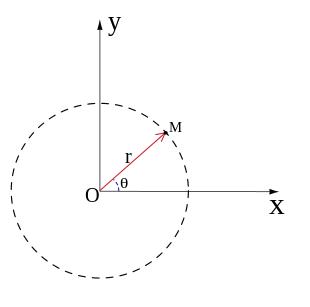
\includegraphics[scale = 0.5]{plan.png}
\end{figure}

\begin{itemize}
  \item{\textbf{Transformation}}
    $ x = r \cos{\theta} , \quad y = r \sin{\theta}$
  \item{\textbf{Élément d'aire}}
    $\dif A = r \dif r \dif\theta$
  \item{\textbf{Gradient}}
    $$\nabla f = \dfrac{\delta f}{\delta r} \Hat{r} + \dfrac{1}{r} \dfrac{\delta f}{\delta \theta}$$

  \item{\textbf{Champ de vecteur}} $F(r,\theta) = F_r(r,\theta) \Hat{r} + F_\theta(r,\theta)\Hat{\theta}$

  \item{\textbf{Divergence}}
    $$
    \nabla \cdot F = \dfrac{\delta F_r}{\delta r}+ \dfrac{1}{r} F_r + \dfrac{1}{r} \dfrac{\delta F_\theta}{\delta \theta}
    $$

  \item{\textbf{Rotationnel}}
    $$
    \nabla \times F=
    \begin{bmatrix}
      \dfrac { \delta { F }_{ \theta } }{ \delta r }  + \dfrac{F_\theta}{r}-\dfrac{1}{r} \dfrac{\delta F_r}{\delta \theta}
    \end{bmatrix}
    \Hat{k}
    $$
\end{itemize}

\subsection{Coordonnées cylindriques polaires}

\begin{figure}[ht!]
  \centering
  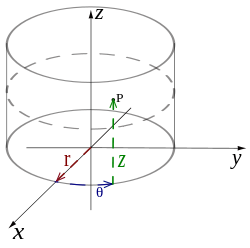
\includegraphics[scale = 0.5]{cylindre.png}
\end{figure}

\begin{itemize}
  \item{\textbf{Transformation}}
    $
    x = r\cos{\theta} , \quad y = r \sin{\theta} , \quad z = z
    $
  \item{\textbf{Élément d'aire (r = a)}}
    $
    dS = a \dif\theta \dif z
    $
  \item{\textbf{Élément de volume}}
    $
    \dif V = r \dif r \dif\theta \dif z
    $
  \item{\textbf{Gradient}}
    $$
    \nabla f = \dfrac{\delta f}{\delta r} \Hat{r} + \dfrac{1}{r} \dfrac{\delta f}{\delta \theta} \Hat{\theta} + \dfrac{\delta f}{\delta z} \Hat{k}
    $$
  \item{\textbf{Champ de vecteur}}
    $
    F(r,\theta, z) = F_r(r,\theta,z) \Hat{r} + F_\theta(r,\theta,z)\Hat{\theta} + F_z (r, \theta , z) \Hat{k}
    $
  \item{\textbf{Divergence}}
    $$
    \nabla \cdot F = \dfrac{\delta F_r}{\delta r}+ \dfrac{1}{r} F_r + \dfrac{1}{r}  \dfrac{\delta F_\theta}{\delta \theta}  + \dfrac{\delta F_z}{\delta z}
    $$
  \item{\textbf{Rotationnel}}
    $$
    \nabla \times F=\frac { 1 }{ r }
    \begin{vmatrix}
      \Hat{r} & r\Hat{\theta} & \Hat{k} \\
      \dfrac{\delta }{\delta r} & \dfrac{\delta }{\delta \theta} & \dfrac{\delta }{\delta z} \\
      F_r & rF_\theta& F_z
    \end{vmatrix}
    $$
\end{itemize}

\subsection{Coordonnées sphériques polaires}

% !! l'image ne correspond pas aux formules !!
\begin{figure}[ht!]
  \centering
  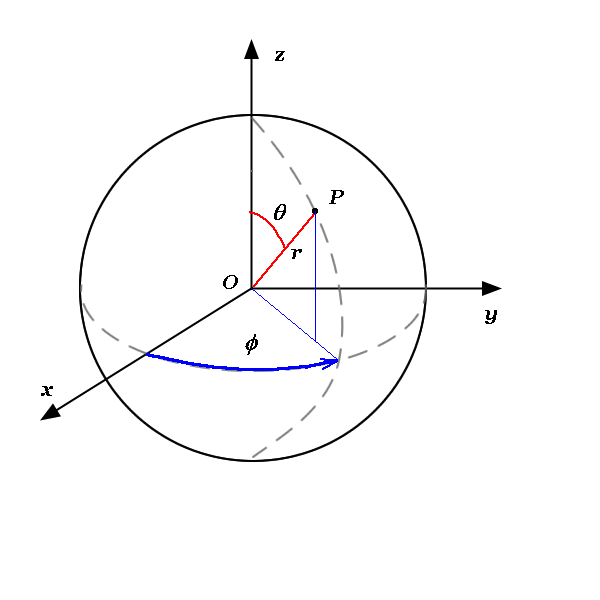
\includegraphics[scale = 0.4]{sphere.png}
\end{figure}


\begin{itemize}
  \item{\textbf{Transformation}}
    $
    x = \rho \sin{\phi}\cos{\theta} ,\quad  y = \rho \sin{\phi} \sin{\theta} ,\quad z = \rho \cos{\phi}
    $\\
    Note : $\phi \in [0,\pi]$ et $\theta \in [0,2\pi]$
  \item{\textbf{Élément d'aire ($\rho = a$)}}
    $
    dS = a^2 \sin{\phi} \dif\theta \dif\phi
    $
  \item{\textbf{Élément de volume}}
    $
    \dif V = \rho^2 \sin{\phi} \dif\rho \dif\phi \dif\theta$
  \item{\textbf{Gradient}}
    $$
    \nabla f = \frac{\delta f}{\delta \rho} \Hat{\rho} + \frac{1 }{\rho} \frac{\delta f}{\delta \phi} \Hat{\Phi} + \frac{1}{\rho \sin{\phi}} \frac{\delta f}{\delta \theta} \Hat{\theta}
    $$
  \item{\textbf{Champ de vecteur}}
    $
    F(\rho, \phi,\theta) = F_r(\rho, \phi,\theta) \Hat{\rho} + F_\phi(\rho, \phi, \theta)\Hat{\phi} + F_\theta (\rho, \phi,\theta) \Hat{\theta}$
  \item{\textbf{Divergence}}
    $$
    \nabla \cdot F = \dfrac{\delta F_\rho}{\delta \rho} +  \dfrac{2}{\rho}F_\rho +  \dfrac{1}{\rho}  \dfrac{\delta F_\phi}{\delta \phi} +  \dfrac{\cot{\phi}}{\rho} F_\phi +  \dfrac{1}{\rho \sin{\phi}}  \dfrac{\delta F_\theta }{\delta \theta }$$
  \item{\textbf{Rotationnel}}
    $$
    \nabla \times F=\frac { 1 }{ \rho^2 \sin{\phi} }
    \begin{vmatrix}
      \Hat{\rho} & \rho\Hat{\Phi} & \rho \sin{\phi}\Hat{\theta} \\
      \dfrac{\delta }{\delta \rho} & \dfrac{\delta }{\delta \phi} & \dfrac{\delta }{\delta \theta} \\
      F_\rho & \rho F_\phi & \rho \sin{\phi} F_\theta
    \end{vmatrix}
    $$
\end{itemize}

\end{document}
